
\graphicspath{{Chapter3/Figs/}}

\setcounter{chapter}{6}
\chapter*{Capítulo 3.} 
\addcontentsline{toc}{chapter}{Capítulo 3}
\setcounter{figure}{0}
\setcounter{table}{0}
\setcounter{section}{0}

{\LARGE Enfoque bioinformático para el estudio de la evolución y biogénesis de miARNs en plantas.}


\section{Introducción.}

En el capítulo anterior vimos que los precursores de plantas pueden ser procesados por cuatro mecanismos con distintas características (Figura \ref{fig:mecanismos}).
Esto contribuye a la complejidad del sistema de procesamiento, respecto al de animales.

Los estudios que dan origen a estos modelos de procesamiento se basan principalmente en datos de secuenciación masiva de ARN en los que se detectan los intermediarios de procesamiento de los distintos precursores.
Como se mostró anteriormente, a partir de los intermediarios de procesamiento es posible definir cuál es el mecanismo al que es sometido cada precursor.

En estudios previos que consideran a los precursores de miARNs en plantas como un solo grupo de moléculas se han encontrado pocos elementos comunes en sus estructuras \citep{Mateos2010}.
En este capítulo, aprovechamos los datos genómicos generados por nuestro laboratorio a partir del estudio del procesamiento de miARNs en plantas, y agrupamos los precursores por mecanismo de procesamiento y estudiamos en detalle a cada precursor en forma individual.
Además, incluimos en el análisis distintas especies de plantas para poder estudiar el procesamiento de miARNs mediante un enfoque evolutivo.

Que los precursores de miARNs en plantas sean procesados de diferentes maneras \citep{Bologna2013}, nos llevó a especular que su patrón de evolución también puede ser diferente y podrían estar vinculados a su mecanismo de procesamiento.
El objetivo es deducir los patrones de los precursores de plantas que sirvan de guía durante el proceso de biogénesis de miARNs.
Es por esto, que elaboramos una estrategia bioinformática para caracterizar la relación entre la evolución de los precursores de miARNs en plantas y los mecanismos de procesamiento determinados previamente.

\section{Resultados y Discusión.}

\subsection{Estrategia bioinformática para el estudio de la evolución y biogénesis de miARNs en plantas.}

La metodología utilizada para el estudio de la evolución y biogénesis de miARNs en plantas se detalla en la Materiales y Métodos (sección \ref{sec:ref_evolution}).
En una primera parte, la utilizamos para estudiar precursores de miARNs conservados en dicotiledóneas. 
Brevemente, la misma consta de los siguientes pasos:

\begin{itemize}
    \item Búsqueda de ortólogos para cada miembro de cada familia de Arabidopsis de  precursores de miARNs conservados en plantas.
    \item Extensión de las secuencias.
    \item Alineamiento de secuencia primaria.
    \item Alineamiento de secuencia teniendo en cuenta estructura secundaria.
    \item Búsqueda de motivos conservados.
    \item Representación gráfica de los precursores.
\end{itemize}

\subsubsection{Búsqueda de ortólogos de precursores de miARNs.}

Las secuencias de los precursores de miARNs en miRBase\footnote{http://mirbase.org} (base de datos biológica que contiene secuencias y anotaciones de miARNs) rara vez son validadas experimentalmente, y de hecho muchas de ellas son el resultado de predicciones computacionales de estructuras en forma de tallo y burbuja que incluye el miARN maduro, pero que no se extiende muchas bases más allá del mismo \cite{Kozomara2014}.
Por esto, los determinantes estructurales pueden no estar incluidos en las secuencias mostradas como precursores en miRBASE, en especial si son procesados desde la base.
Por lo tanto, empezamos nuestro análisis con una definición arbitraria de los precursores de plantas incluyendo 150 nt fuera del par miARN/miARN*.
En ese sentido, extendimos la secuencia de los precursores para el posterior análisis utilizandos datos genómicos de plantas extraídos de Phytozome\footnote{http://phytozome.jgi.doe.gov} para 30 especies de dicotiledoneas.

En segundo lugar, para cada miembro de cada familia de \textit{A. thaliana} no es trivial asignarle un ortólogo en otra especie teniendo en cuenta la anotación de miRBase.
Por esto, realizamos una búsqueda de ortólogos para cada miembro de cada familia de \textit{A. thaliana} utilizando como criterio la técnica de Blast recíproco.
Esta técnica consiste en utilizar Blast cruzado para predecir ortólogos putativos (Ver Materiales y Métodos sección \ref{sec:reciprocal_blast}).

%~ Para la mayoría de los miembros de cada familia de precursores pudimos detectar ortólogos en otras especies. 
%~ Teniendo en cuenta las 30 dicotiledóneas utilizadas en este estudio, en promedio, se encontraron ortólogos para cerca de 20 especies para cada precursor de miARN de \textit{A. thaliana} (Figura \ref{fig:dicots_species}).

%~ \begin{figure}[htbp!]
    %~ \centering    
    %~ 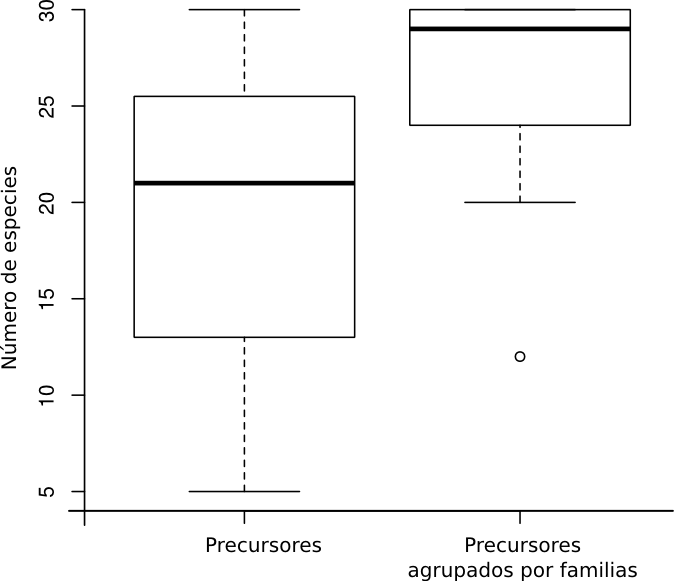
\includegraphics[width=.5\textwidth]{dicots_species.png}
    %~ \caption[Ortólogos detectados en precursores de plantas]{
    %~ \textbf{Ortólogos detectados en precursores de plantas}
    %~ Esta figura muestra la distribución de la cantidad de especies donde se encuentran ortólogos de precursores de miARNs.
    %~ A la izquierda se muestra la distribución de especies por miembro de familias de precursores de miARNs donde se detecta el ortólogo de \textit{A. thaliana}.
    %~ A la derecha se agruparon todos los miembros de una misma familia y se muestra la distribución de la cantidad de especies donde se detecta un ortólogo de \textit{A. thaliana}
    %~ }
    %~ \label{fig:dicots_species}
%~ \end{figure}

Algunos familias de miARNs se han diversificado durante la evolución, donde en algunas especies un miARN puede encontrarse como un único gen y en otras especie el mismo miARN puede encontrarse en múltiples miembros.
Por ejemplo, el miR396 en Arabidopsis está constituido por dos miembros, miR396a y miR396b mientras que en en el caso de arroz existen 8 miembros, nombrados del miR396a al miR396h.
Este variación en el número de genes de miARNs en distintas especies implica que no necesariamente existe un ortólogo a un determinado miARN de Arabidopsis en cada una de las especies.
Sin embargo, no podemos descartar que estemos perdiendo de encontrar miARNs ortólogos por la propia limitación en la búsqueda que hacemos utilizando el blast recíproco.

%~ Por esto, agrupamos a los miembros por familias y vimos la distribución de la cantidad de especies donde se detecta un ortólogo de los precursores de miARNs pertenecientes a \textit{A. thaliana}.
%~ Y agrupando por familia, vimos un alto número de especies promedio detectadas para la mayoría de las familias de miARNs (Figura \ref{fig:dicots_species}).
%~ Es decir que con esta estrategia pudimos detectar ortólogos en la mayoría de las especies, para al menos un miembro de todas las familias de miARNs conservados en dicotiledóneas. 

\subsubsection{Alineamiento de los precursores en base a su secuencia primaria.}

Como resultado de la búsqueda de ortólogos de precursores de miARNs de los 93 precursores de Arabidopsis encontramos 1819 precursores en total en las 30 especies de dicotiledóneas.
En la Figura \ref{fig:miR172a_rnafold} se muestran las estructuras secundarias de los ortólogos del precursor de miR172a utilizando el programa RNAfold \citep{pmid22115189}.
Como puede verse, si bien hay una similitud entre las estructuras es difícil deducir información concreta a partir de esta Figura.

A continuación, comenzamos con los alineamientos múltiples de cada miembro de las familias de precursores de miARNs conservadas en dicotiledóneas.
Primero, realizamos el alineamiento en base a su secuencia primaria utilizando la herramienta T-Coffee \citep{pmid10964570}.

En la Figura \ref{fig:miR172a_tcoffee} se muestra el alineamiento del precursor del miR172a en distintas especies, coloreado en base a la conservación evolutiva de la secuencia primaria.
Se puede observar que el miR172a maduro y el miR172a* están muy conservados en las distintas especies, pero además se puede ver una cola de conservación hacia la izquierda del miARN y hacia la derecha del miARN* (Figura \ref{fig:miR172a_tcoffee} en líneas de puntos).


\begin{landscape}
    \begin{figure}[htbp!] 
        \centering    
        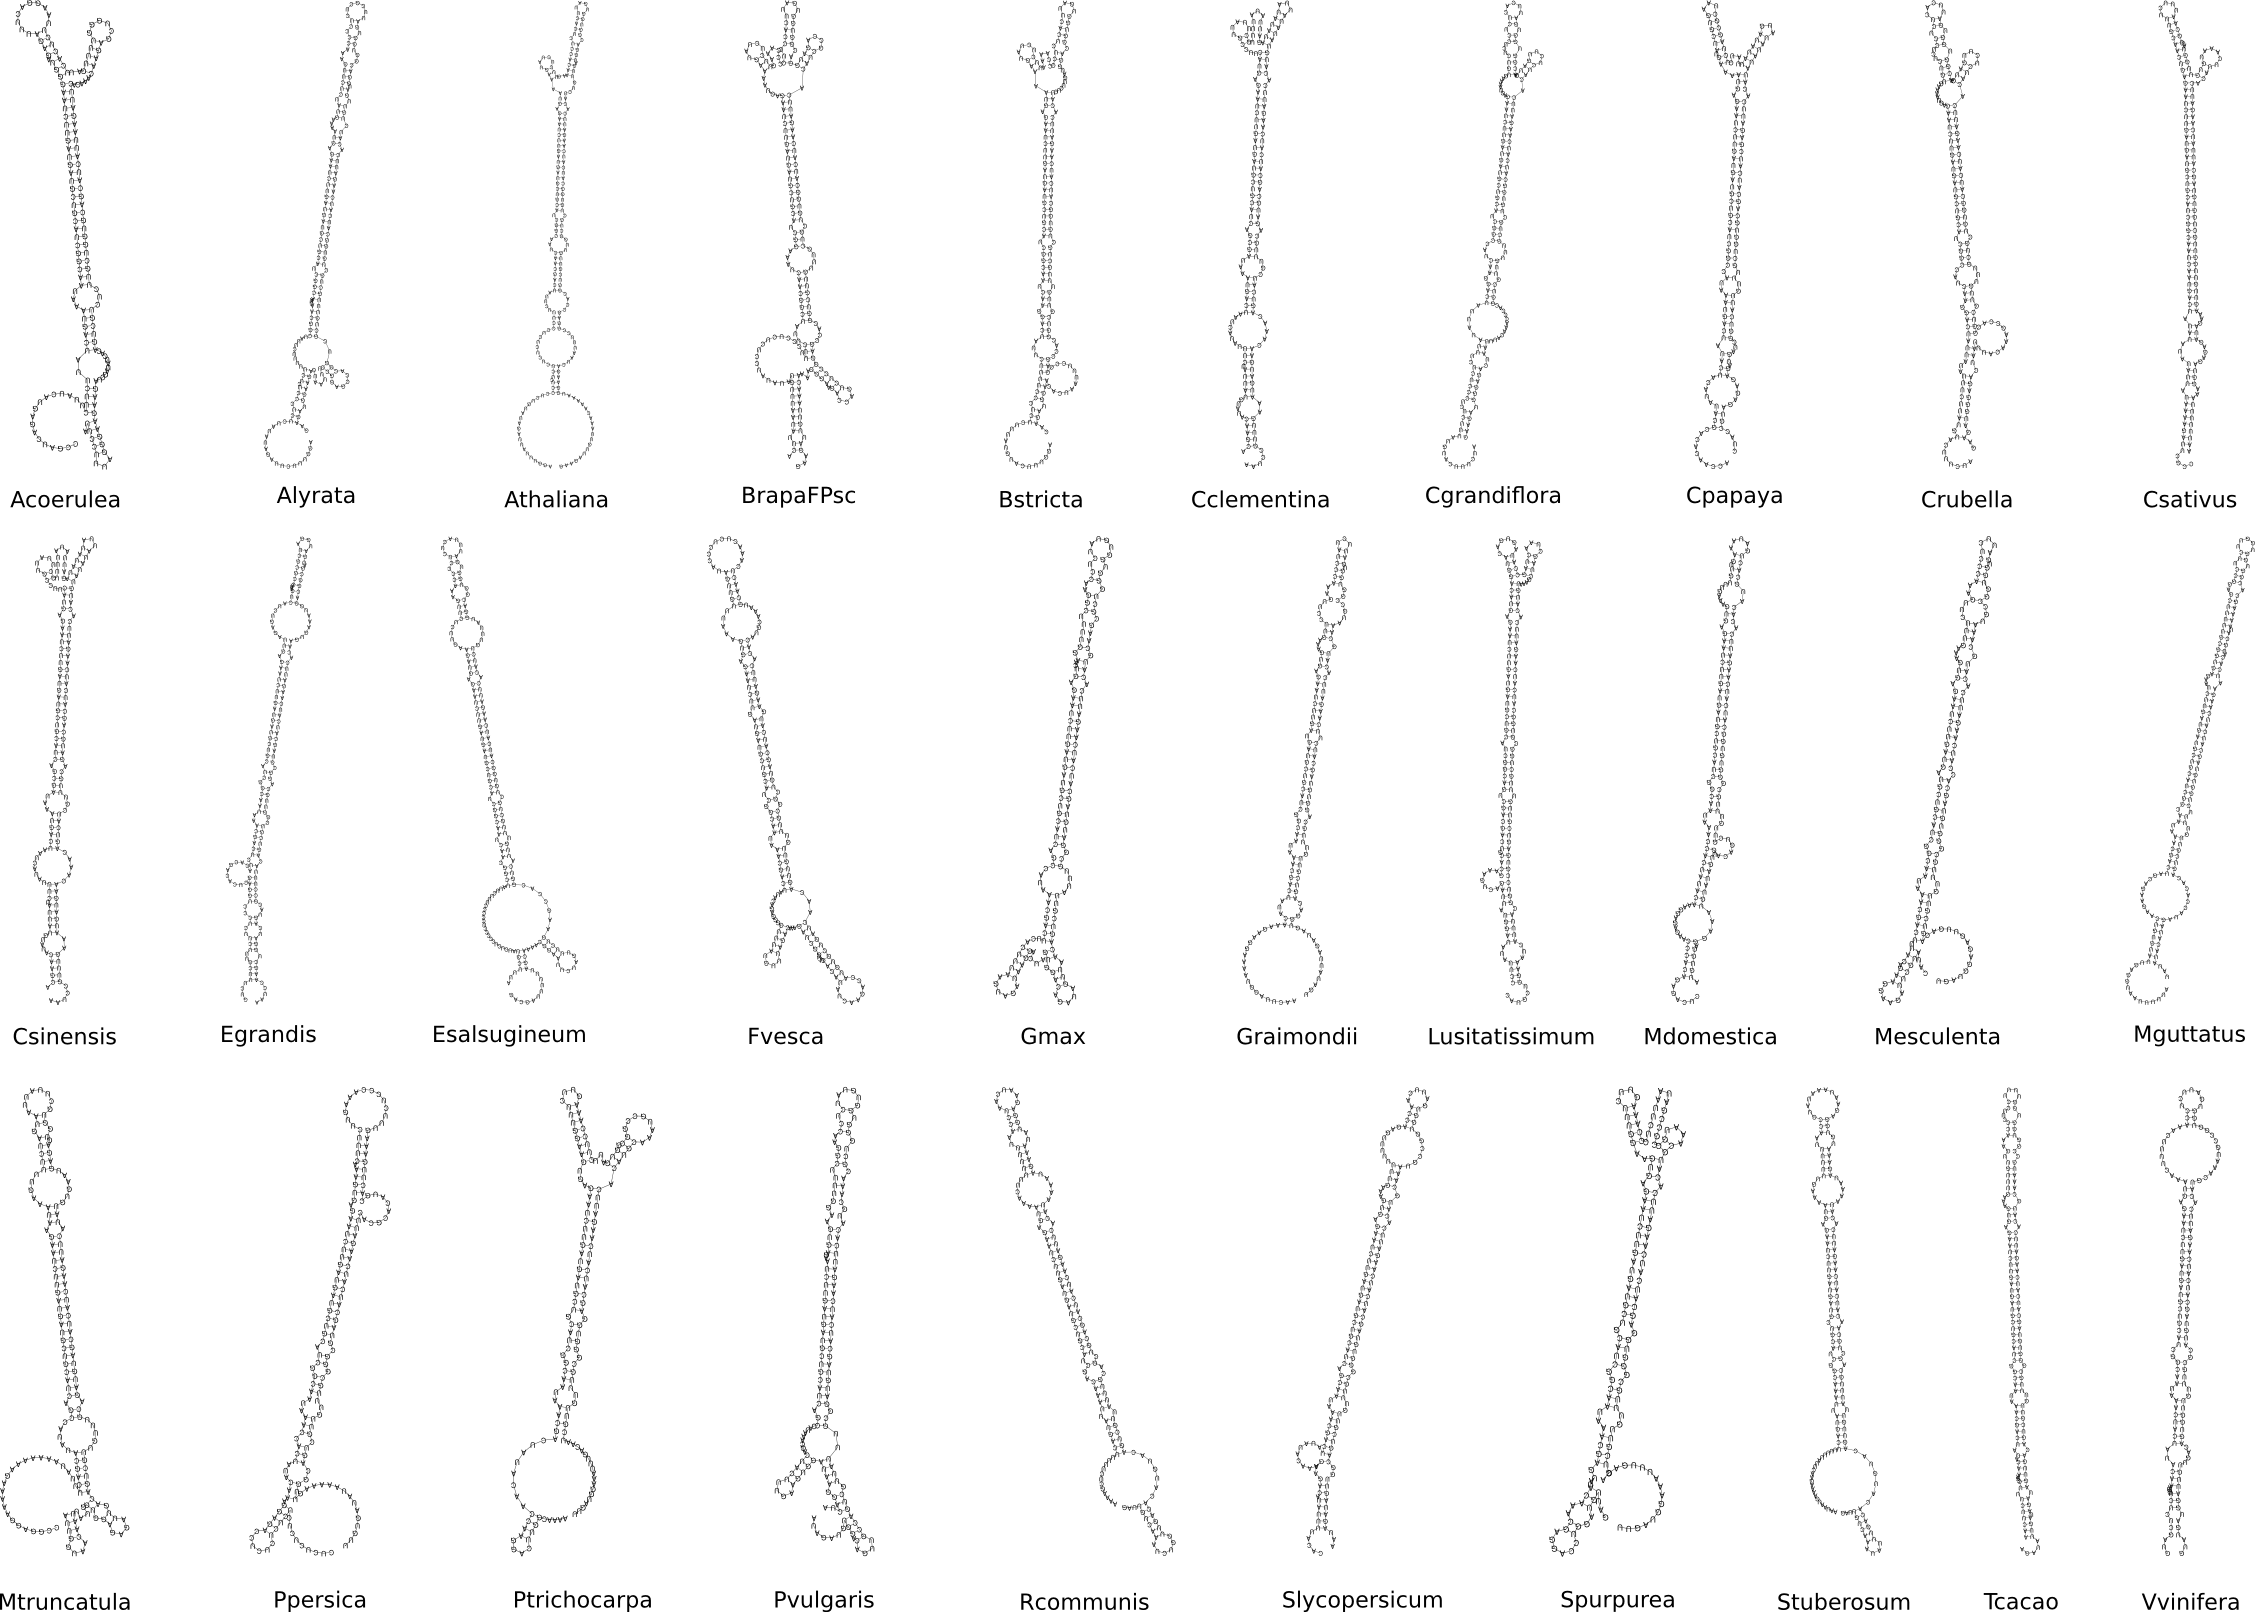
\includegraphics[width=1.4\textwidth]{miR172a_rnafold.png}
        \caption[Estructura secundaria del miR172a en distintas especies]{
        \textbf{Estructura secundaria del miR172a en distintas especies.}
        Se muestra la estructura secundaria de los precursores del miR172a en distintas especies, calculados con la herramienta RNAfold.
        Se puede observar que existe un patrón estructural que comparten los precursores, en la región inmediata por debajo del dúplex miARN/miARN*.
        }
        \label{fig:miR172a_rnafold}
    \end{figure}
\end{landscape}

\begin{landscape}
    \begin{figure}[htbp!] 
        \centering    
        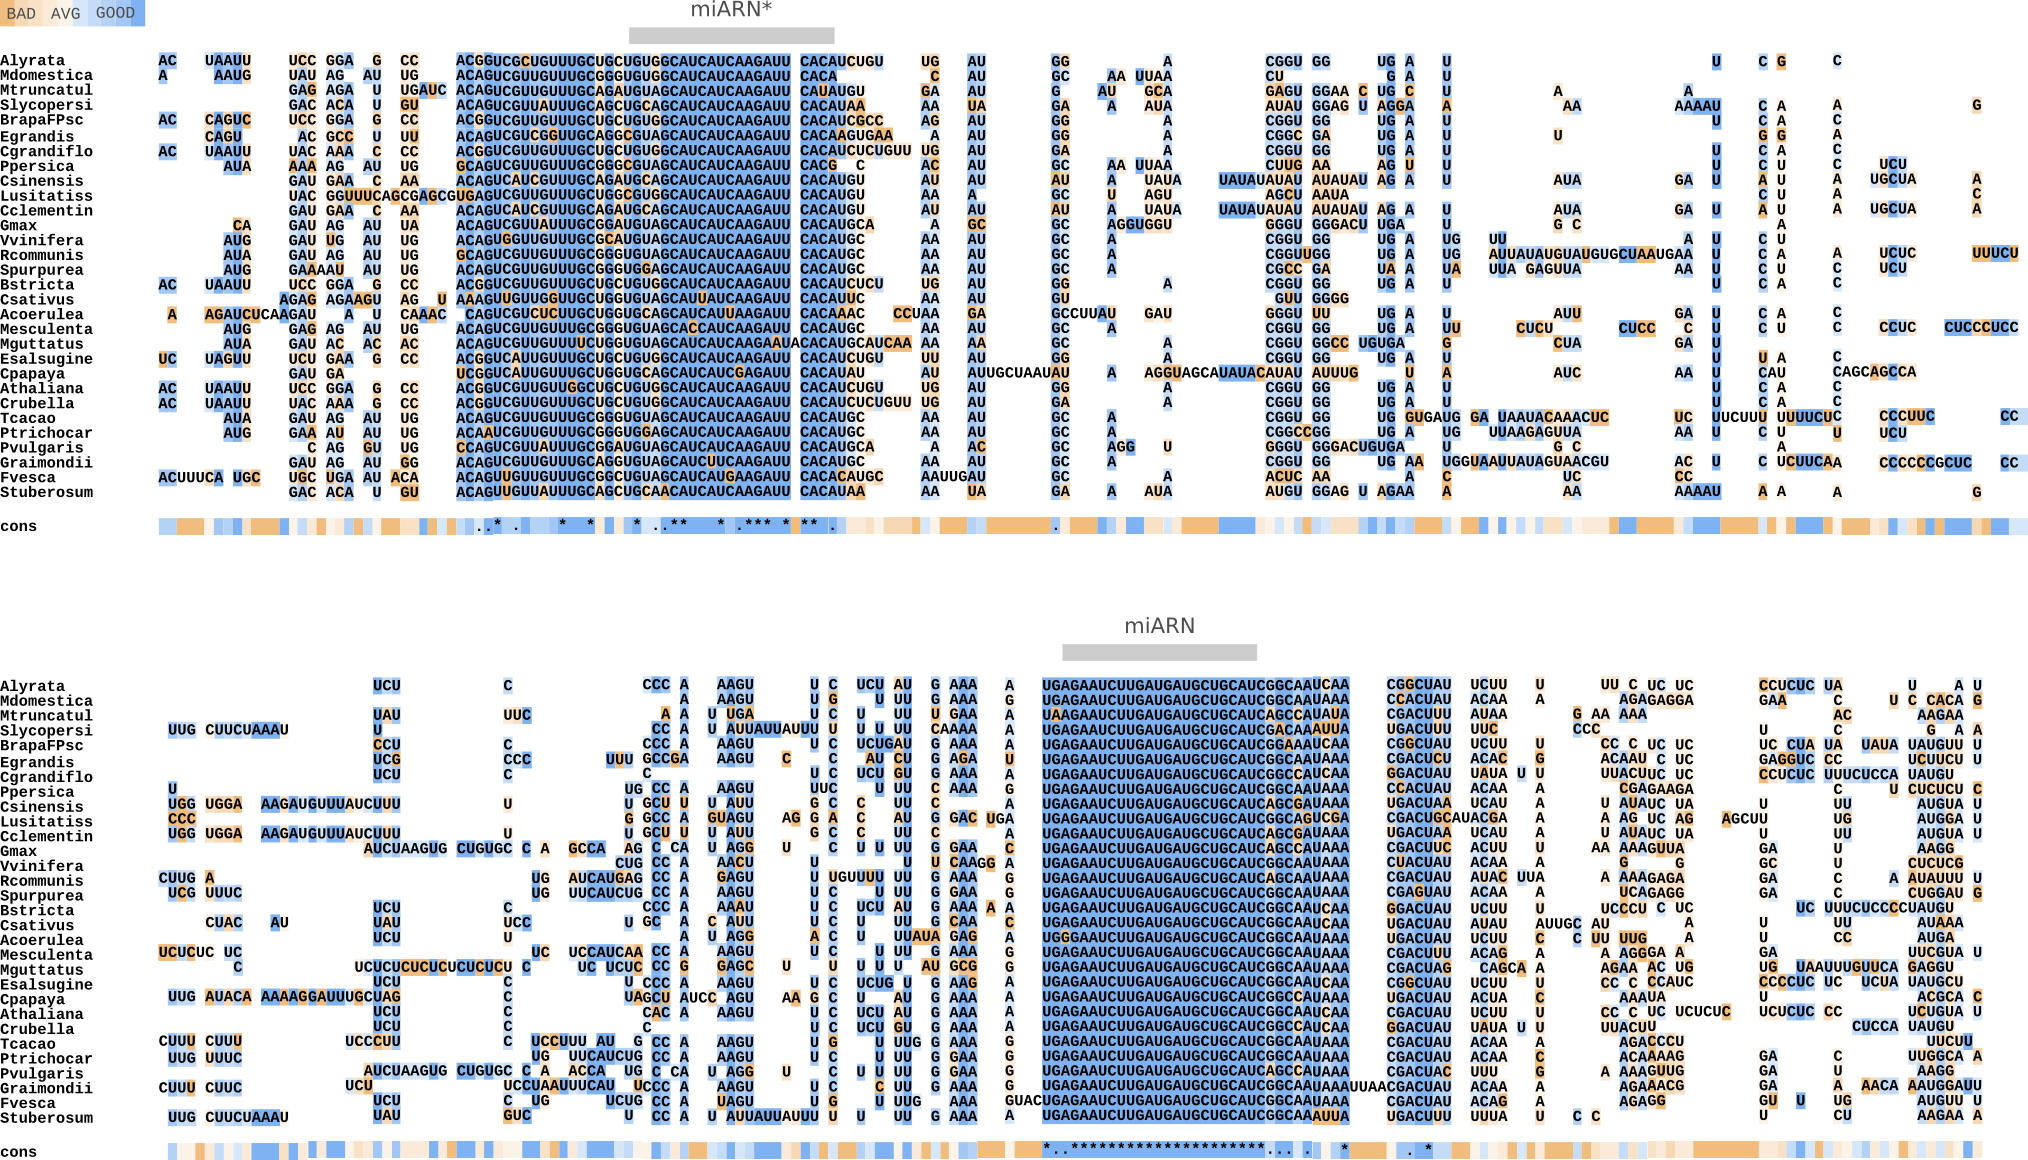
\includegraphics[width=1.4\textwidth]{miR172a_tcoffee.png}
        \caption[Alineamiento del precursor del miR172a.]{
        \textbf{Alineamiento del precursor del miR172a.}
        Se muestra el alineamiento del precursor del miR172a en distintas especies. 
        En colores se muestra la conservación de la secuencia primaria, donde azul más oscuro denota mayor conservación y naranja menor conservación.
        Se muestran $\sim$60 bases por debajo del dúplex miARN/miARN* y los alineamientos están separados en dos líneas para una mejor representación.
        Se puede observar conservación en el miARN y el miARN*.
        Además, se marca en línea de puntos una cola de conservación.}
         \label{fig:miR172a_tcoffee}
    \end{figure}
\end{landscape}


Esta cola de conservación se corresponde al tallo inferior del precursor.
Sin embargo, esta forma de visualización no hace fácil correlacionar conservación con estructura secundaria.
%~ Luego realizamos nuevamente los alineamientos pero considerando la estructura secundaria de los precursores, y para esto utilizamos la herramienta R-Coffee \citep{pmid18292307}.

Después de estos primeros análisis, llegamos a la conclusión de que el análisis de la conservación evolutiva de cada precursor era valioso ya que permitía identificar regiones conservadas que tienen una función en el procesamiento.
Sin embargo, también notamos que la forma de representación de esta información no era del todo conveniente, en especial, teniendo en cuenta la cantidad de precursores estudiados en esta parte del trabajo de Tesis.


\subsubsection{Diseño de una implementación gráfica para la visualización integral de los precursores.}

Para poder reconocer fácilmente la región conservada dentro del precursor y poder analizar más en detalle estos patrones de conservación, decidimos agrupar toda esta información 
generada a partir de los alineamientos de secuencia primaria y estructura secundaria en un gráfico circular como se muestra en la Figura \ref{fig:miR172a_circos}.
Estos gráficos se hicieron utilizando el paquete Circos \citep{pmid19541911}, que adaptamos para visualizar los precursores de miARNs.
 
En dicha Figura, se muestra el Circos del precursor del miR172a a modo de ejemplo.
Para representar el precursor, se tomaron 60 nt por debajo del dúplex miARN/miARN*.
En el anillo exterior se representa, en colores azules y marrones, el grado de conservación de la secuencia consenso a partir de los alineamientos en base a su secuencia primaria.
Además, se muestran las bases del precursor de \textit {A. thaliana} que corresponden a la posición consenso.
Luego en el anillo interior se representa, mediante un histograma, la frecuencia de bases apareadas y desapareadas para cada posición del precursor en las distintas especies, donde una barra verde indica que la posición tiende a estar apareada formando una estructura secundaria, mientras que la barra violeta indica que la base tiende a estar desapareada. 
Con líneas de distinto espesor se muestra la interacción entre pares de bases del precursor considerando la estructura secundaria. 
Finalmente por fuera del anillo exterior se marca la secuencia del miARN y miARN*.

Estos gráficos denominados Circos, los adaptamos y los realizamos, para visualizar de manera simple los precursores de miARNs en distintas especies de plantas.
Y luego fueron utilizados para caracterizar la relación entre los patrones de conservación y los mecanismos de procesamiento en plantas determinados previamente.


\begin{figure}[htbp!] 
    \centering    
    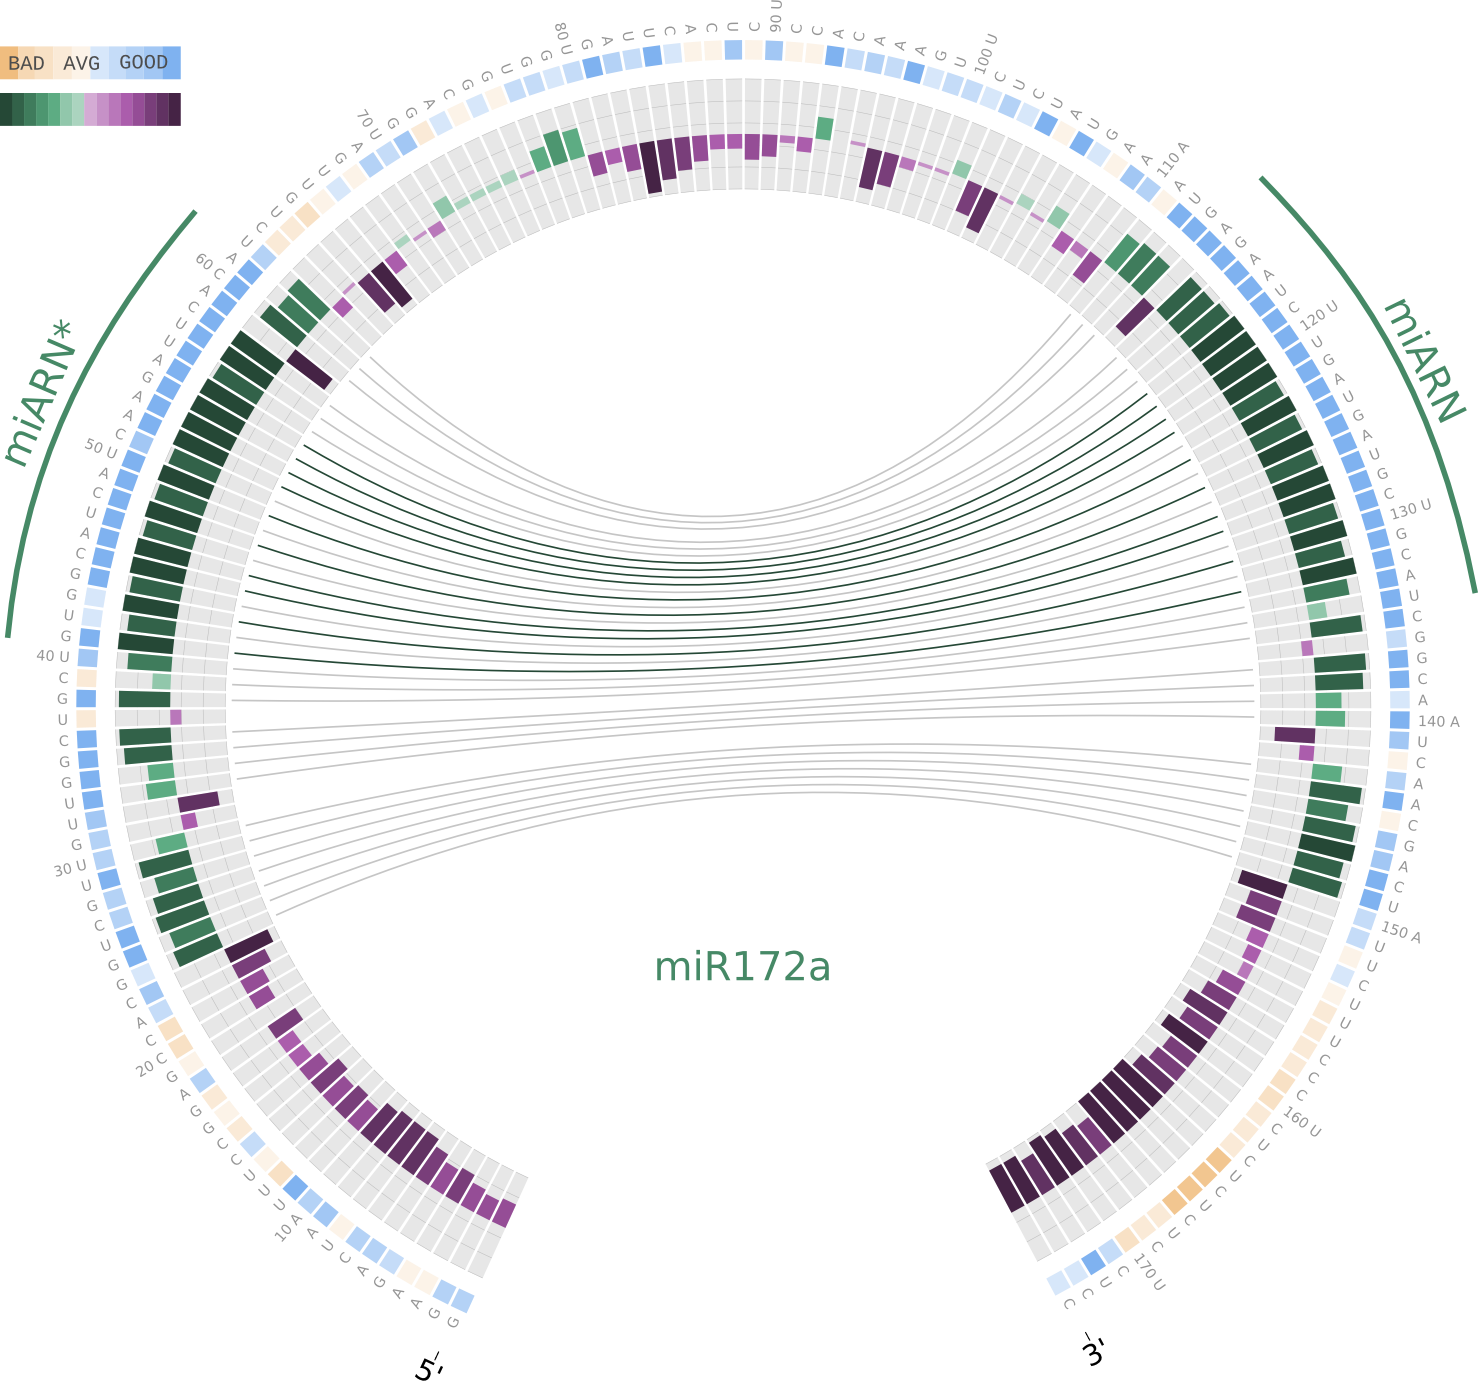
\includegraphics[width=1\textwidth]{miR172a_circos.png}
    \caption[Circos del miR172a]{
    \textbf{Circos del miR172a.}
En el anillo exterior se representa en colores el grado de conservación de la secuencia consenso a partir de los alineamientos en base a su secuencia primaria.
Además, se muestran las bases del precursor de \textit {A. thaliana}.
Luego en el anillo interior se representa, mediante un histograma, la frecuencia de bases apareadas y desapareadas para cada posición del precursor en las distintas especies, donde una barra verde indica que la posición tiende a estar apareada formando una estructura secundaria, mientras que la barra violeta indica que la base tiende a estar desapareada. 
Con líneas de distinto espesor se muestra la interacción de las bases del precursor considerando la estructura secundaria. 
Fuera del anillo exterior se marca la secuencia del miARN y miARN*.
   }
     \label{fig:miR172a_circos}
\end{figure}


\subsection{Visualización por Circos de precursores que se procesan desde la base.}

De acuerdo al análisis de las bibliotecas SPARE, en los precursores con un mecanismo corto de base a loop, un loop interno seguido por un tallo inferior de $\sim$15nt especifica la posición del primer corte por debajo del miARN.
El segundo corte procede a una distancia fija de $\sim$21 nt desde la posición del primer corte.

Para la mayoría de los precursores procesados con este mecanismo, pudimos observar el mismo patrón de conservación de estructura primaria y similares patrones de estructura secundaria que se muestra para el caso del precursor del miR172a (Figura \ref{fig:miR172a_circos}) y del precursor del miR390a (Figura \ref{fig:miR390a_circos}).
En ambos casos los gráficos representan, ortólogos en las 30 especies utilizadas.
También, se pudo observar que la región con mayor conservación coincide con el dúplex miARN/miARN*, pero además, se puede ver una región conservada por debajo del dúplex, que coincide con el tallo inferior del precursor.
Se puede observar que esta región esta relativamente conservada a nivel de estructura primaria como secundaria.

\begin{figure}[htbp!] 
    \centering    
    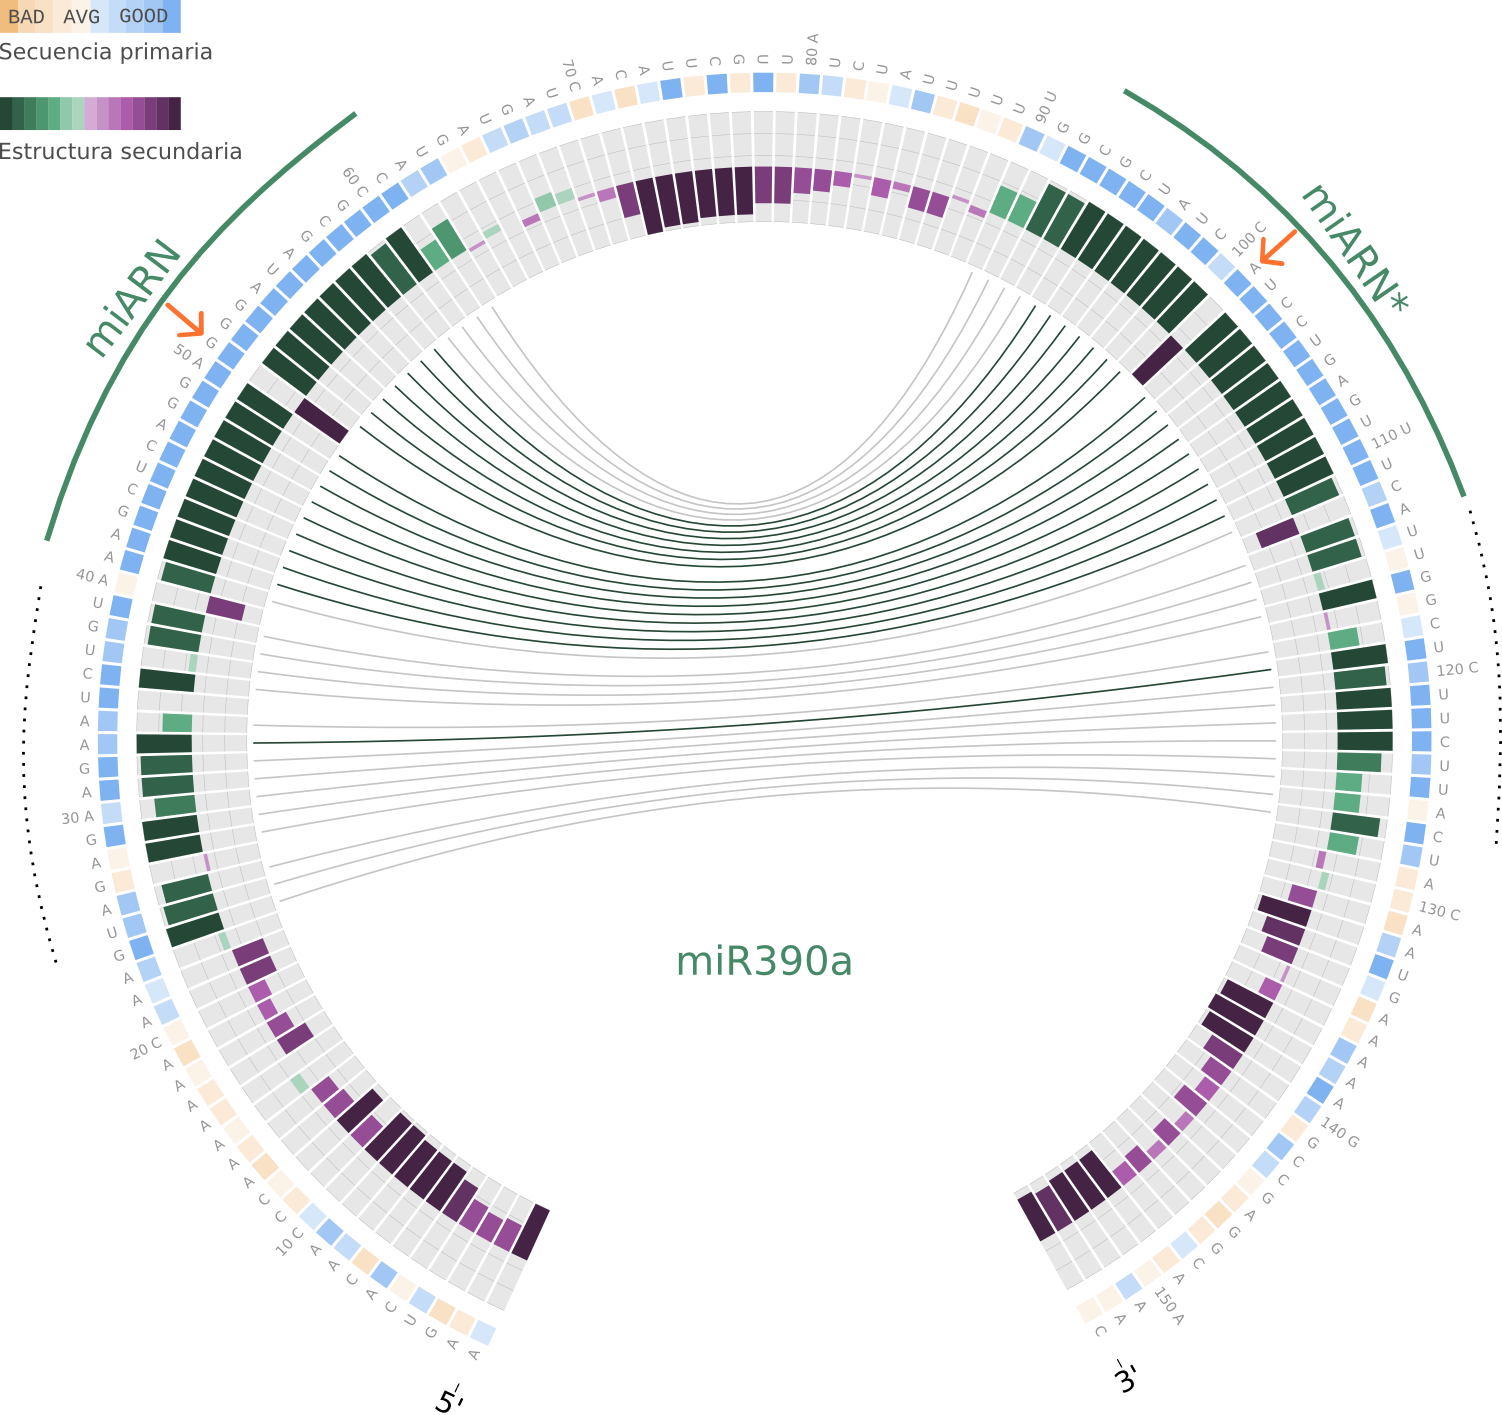
\includegraphics[width=1\textwidth]{miR390a_circos.png}
    \caption[Circos del miR172a]{
    \textbf{Circos del miR390a.}
    Se puede observar que la región con mayor conservación coincide con el dúplex miARN/miARN*.
    Además, se puede observar una región conservada por debajo del dúplex, que coincide con el tallo inferior.
    }
     \label{fig:miR390a_circos}
\end{figure}

Otra ventaja de esta forma de representar a los precursores con la conservación entre especies, es que visualmente se puede reconocer fácilmente las posiciones donde existen ``mismatches'' conservados. 
Por ejemplo, en el Circos del miR172, se puede observar que la primera base del miARN tiende a estar desapareada junto con la posición 19 del miARN* (Figura \ref{fig:miR172a_circos}, flecha naranja). 
Esta interacción es A-A y se mantiene sin variaciones en todas las especies analizadas (Figura \ref{fig:miR172a_circos}).
Un caso similar detectamos para el miR390a (Figura \ref{fig:miR390a_circos}, flecha naranja).

Esto podría ser interesante estudiarlo en detalle, donde se podría generar un precursor mutante con esas bases en particular estén apareadas y luego ver si esto afecta o no el procesamiento del precursor.  
\newpage


\subsection{Visualización por Circos de precursores que se procesan desde la base en forma secuencial.}

En estos precursores, con un mecanismo secuencial de base a loop, el primer corte procede como en los precursores cortos de base a loop, pero luego son necesario dos cortes más para liberar el miARN, generando en el proceso niveles bajos de ARN pequeños adicionales \citep{Bologna2013}.
Este es el caso de algunos miembros de la  familias del miR169, que tiene en total 14 miembros siendo la familia más grande de \textit{A. thaliana}.
Un estudio en detalle de los precursores del miR169b/d/e/f/g mostró que los sitios de cortes del precursor estaban localizados 21 nt por debajo del lado proximal del dúplex miARN/miARN*.
Esta es la distancia esperada entre dos cortes de DCL1, sugiriendo que estos precursores eran procesados por más de dos cortes de la encima \citep{Bologna2013}.

Además. la familia del miR394 también es procesada de la misma manera y comparten similares patrones de estructura secundaria, donde se ve el tallo inferior largo bien estructurado (Figura \ref{fig:seqBTL_circos} B).
Si observamos el patrón de conservación de secuencia primaria podemos ver que la región del dúplex miARN/miARN* está muy conservada, pero además podemos observar que debajo del dúplex existe otra región conservada y estructurada, que coincide con el tallo inferior largo estructurado que presentan estos precursores (Figura \ref{fig:seqBTL_circos}).
Es decir, que en estos precursores podemos también correlacionar su procesamiento con la conservación evolutiva.

\begin{landscape}
    \begin{figure}[htbp!] 
        \centering    
        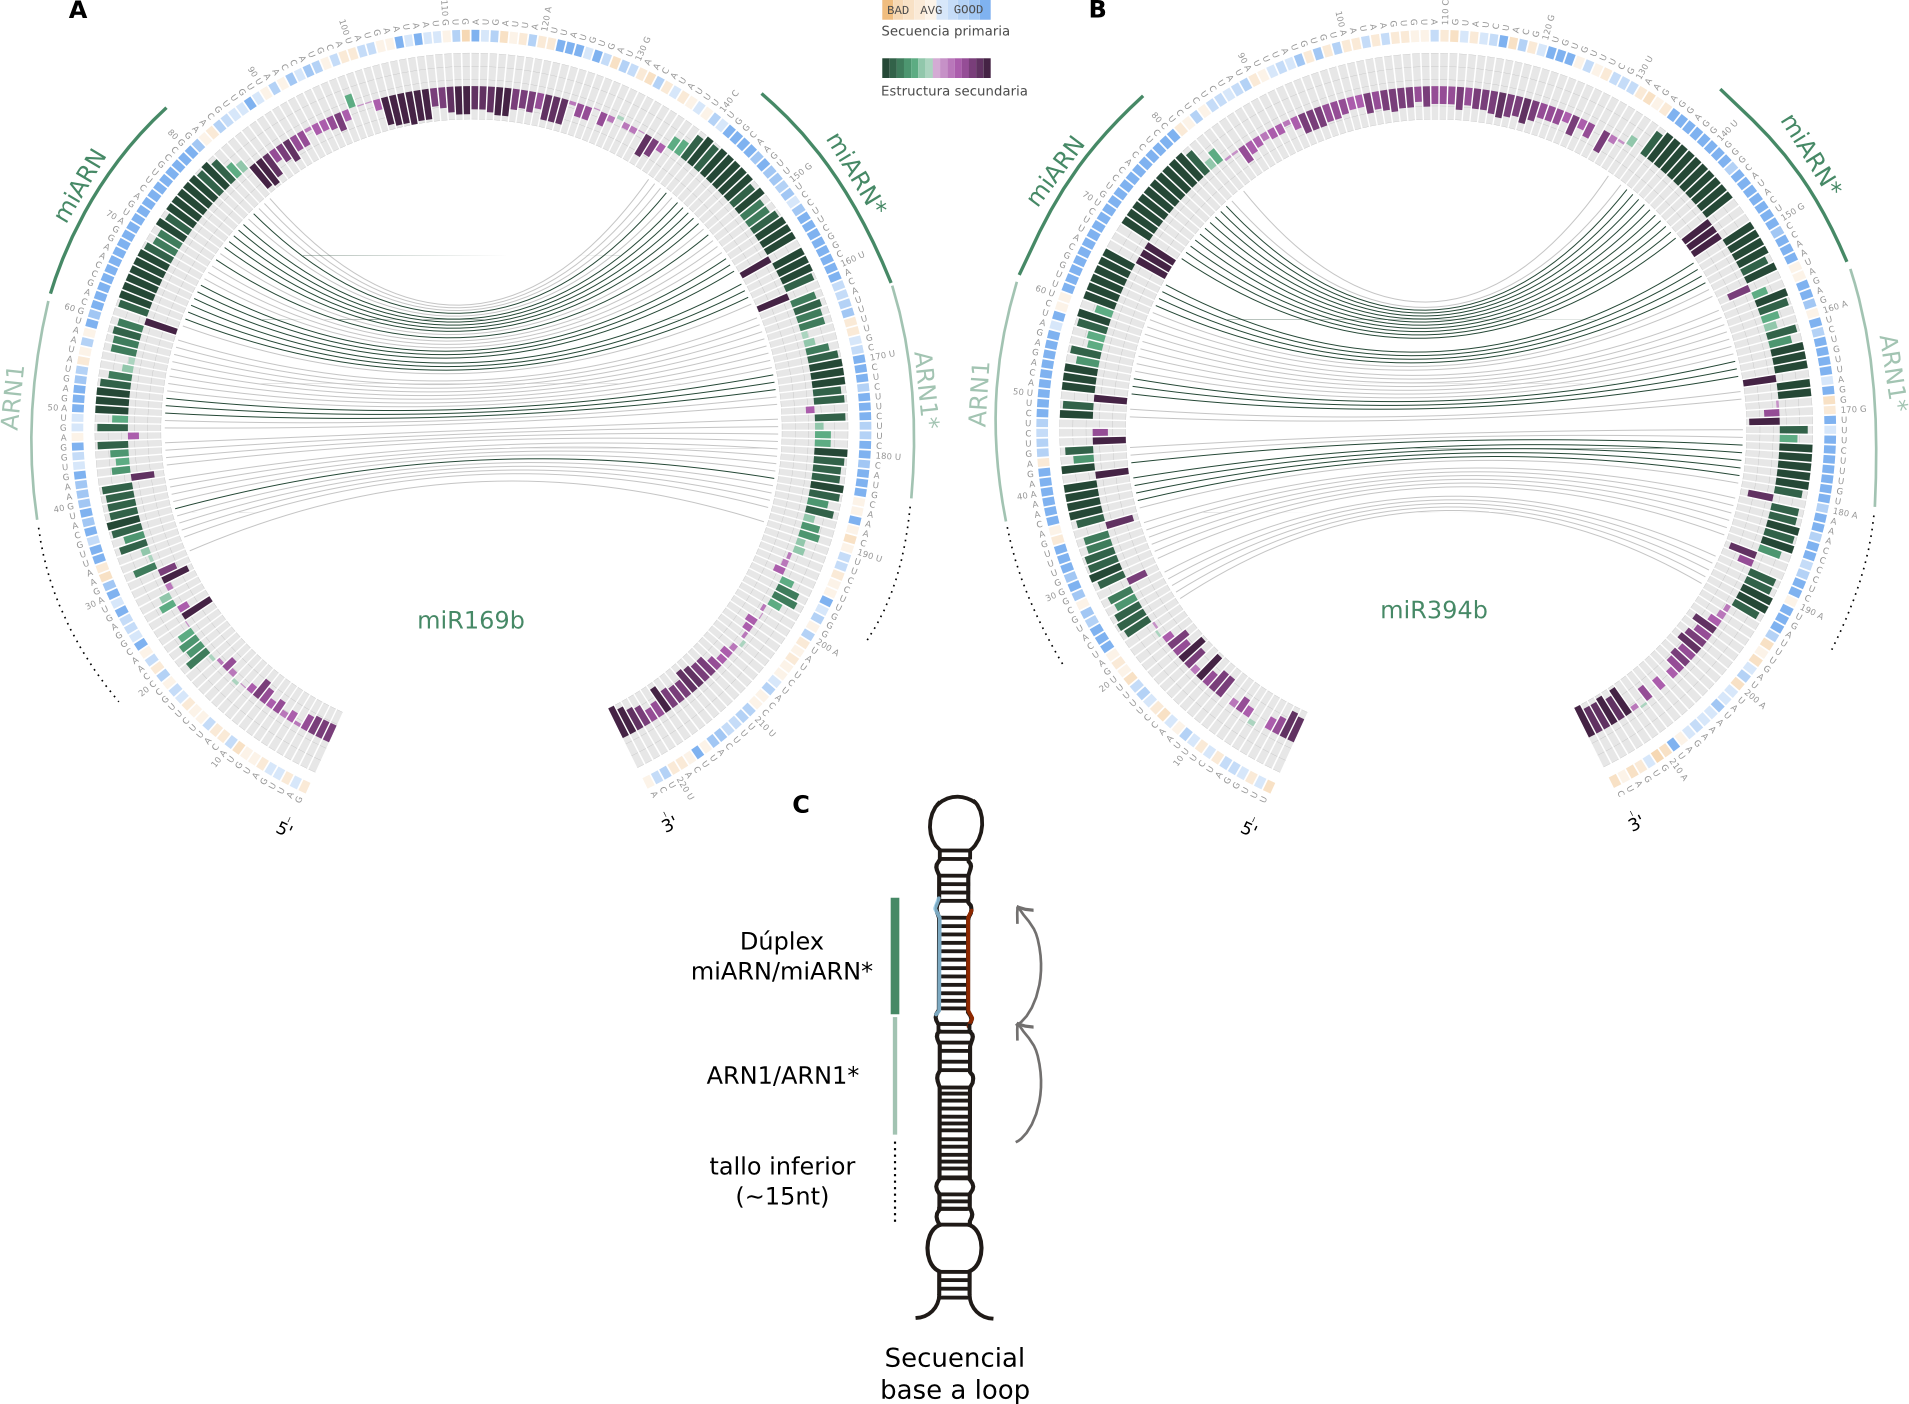
\includegraphics[width=1.3\textwidth]{seqBTL_circos.png}
        \caption[Circos de precursores con mecanismos de procesamientos secuenciales de base a loop]{
        \textbf{Circos de precursores con mecanismos de procesamientos secuenciales de base a loop}
		 \textbf{(A)} Circos del precursor del miR169b.
		 \textbf{(B)} Circos del precursor del miR394b.
		 \textbf{(C)} Estructura de precursores procesados secuenciales de base a loop.
		 En \textbf{(A)} y \textbf{(B)} se puede observar que la región del dúplex miARN/miARN* está muy conservada, pero además podemos observar que debajo del dúplex existe otra región conservada que coincide con el tallo inferior largo.
        Con líneas verde fuera del Circos se muestra la región que corresponde al miARN y al miARN*. 
        Con líneas verde claro fuera del Circos se muestran otros ARN pequeños  generados a partir del primer y segundo corte por DCL1.
        Con líneas de puntos se muestra fuera del Circos la región que corresponde al tallo inferior de $\sim$15nt.
		}
         \label{fig:seqBTL_circos}
    \end{figure}
\end{landscape}


\subsection{Visualización por Circos de precursores que se procesan de arriba cortos.}

En los precursores con un mecanismo cortos de loop a base, el procesamiento es guiado por un tallo superior, y son necesarios dos cortes para liberar el miARN maduro.
La región terminal de estos precursores tienen una largo conservado de $\sim$42, donde incluye un loop pequeño \citep{Bologna2013} a diferencia de los precursores procesados de base a loop, donde esta región es variable en tamaño, como vimos en el capítulo anterior.

En este caso mostramos los Circos para el precursor del miR157a, que fue encontrado en 30 especies, y para el precursor del miR160a también encontrado en 30 especies (Figura \ref{fig:srLTB_circos}). 
En los precursores que se procesan cortos de base a loop observamos que presentan una región conservada que corresponde al tallo superior además de la región que comprende al dúplex miARN/miARN* (Figura \ref{fig:srLTB_circos}).
A diferencia de los precursores que se procesan de la base al loop, estos precursores no presentan el tallo inferior ni estructurado ni conservado y esto se puede observar en ambos casos; en el miR157a (Figura \ref{fig:srLTB_circos} A) y del miR160a (Figura \ref{fig:srLTB_circos} B).


%~ Este patrón de conservación, difiere con el patrón observado para los precursores secuenciales que se procesan desde la base.
%~ JP me puso estás seguro? Como no lo estoy lo eliminé

\begin{landscape}
    \begin{figure}[htbp!] 
        \centering    
        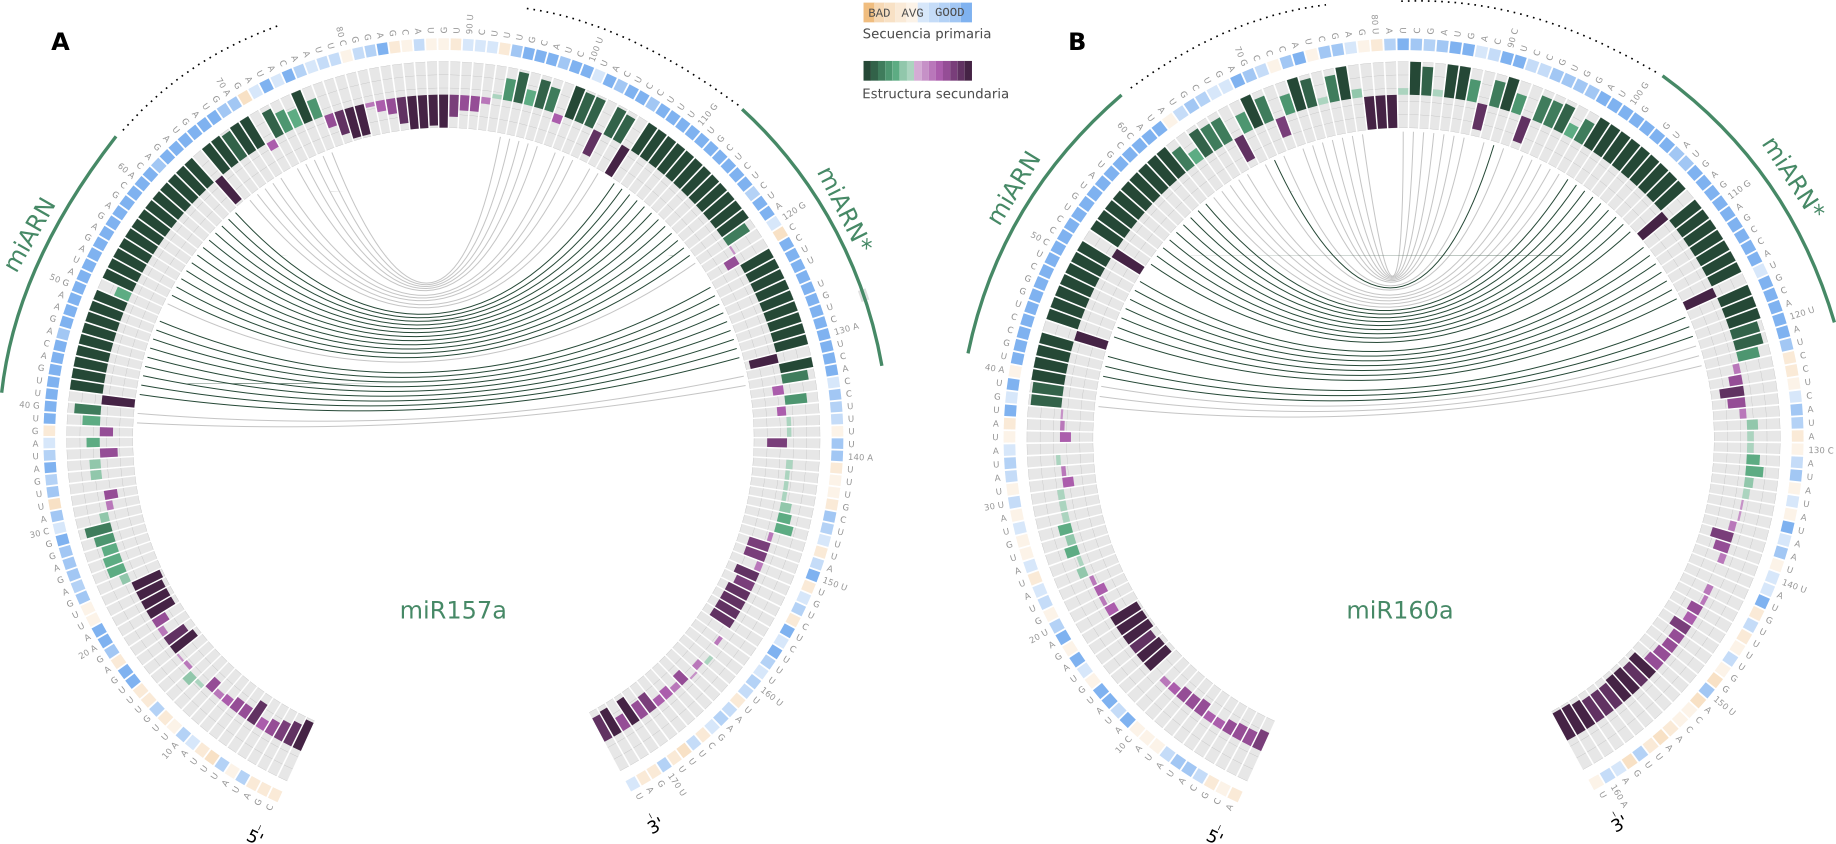
\includegraphics[width=1.4\textwidth]{srLTB_circos.png}
        \caption[Circos de precursores con mecanismos de procesamientos cortos de loop a base]{
        \textbf{Circos de precursores con mecanismos de procesamientos cortos de loop a base}
		 \textbf{(A)} Circos del precursor del miR157a.
		 \textbf{(B)} Circos del precursor del miR160a.
		 \textbf{(C)} Estructura de precursores procesados cortos de loop a base.
		 En \textbf{(A)} y \textbf{(B)} se puede observar que los otros ARNs pequeños están conservados de la misma manera que el miARN y el miARN*.
        Con líneas verde fuera del Circos se muestra la región que corresponde al miARN y al miARN*. 
		Con líneas de puntos se muestra fuera del Circos la región que corresponde al tallo superior.

		}
         \label{fig:srLTB_circos}
    \end{figure}
\end{landscape}


\begin{landscape}
    \begin{figure}[htbp!] 
        \centering    
        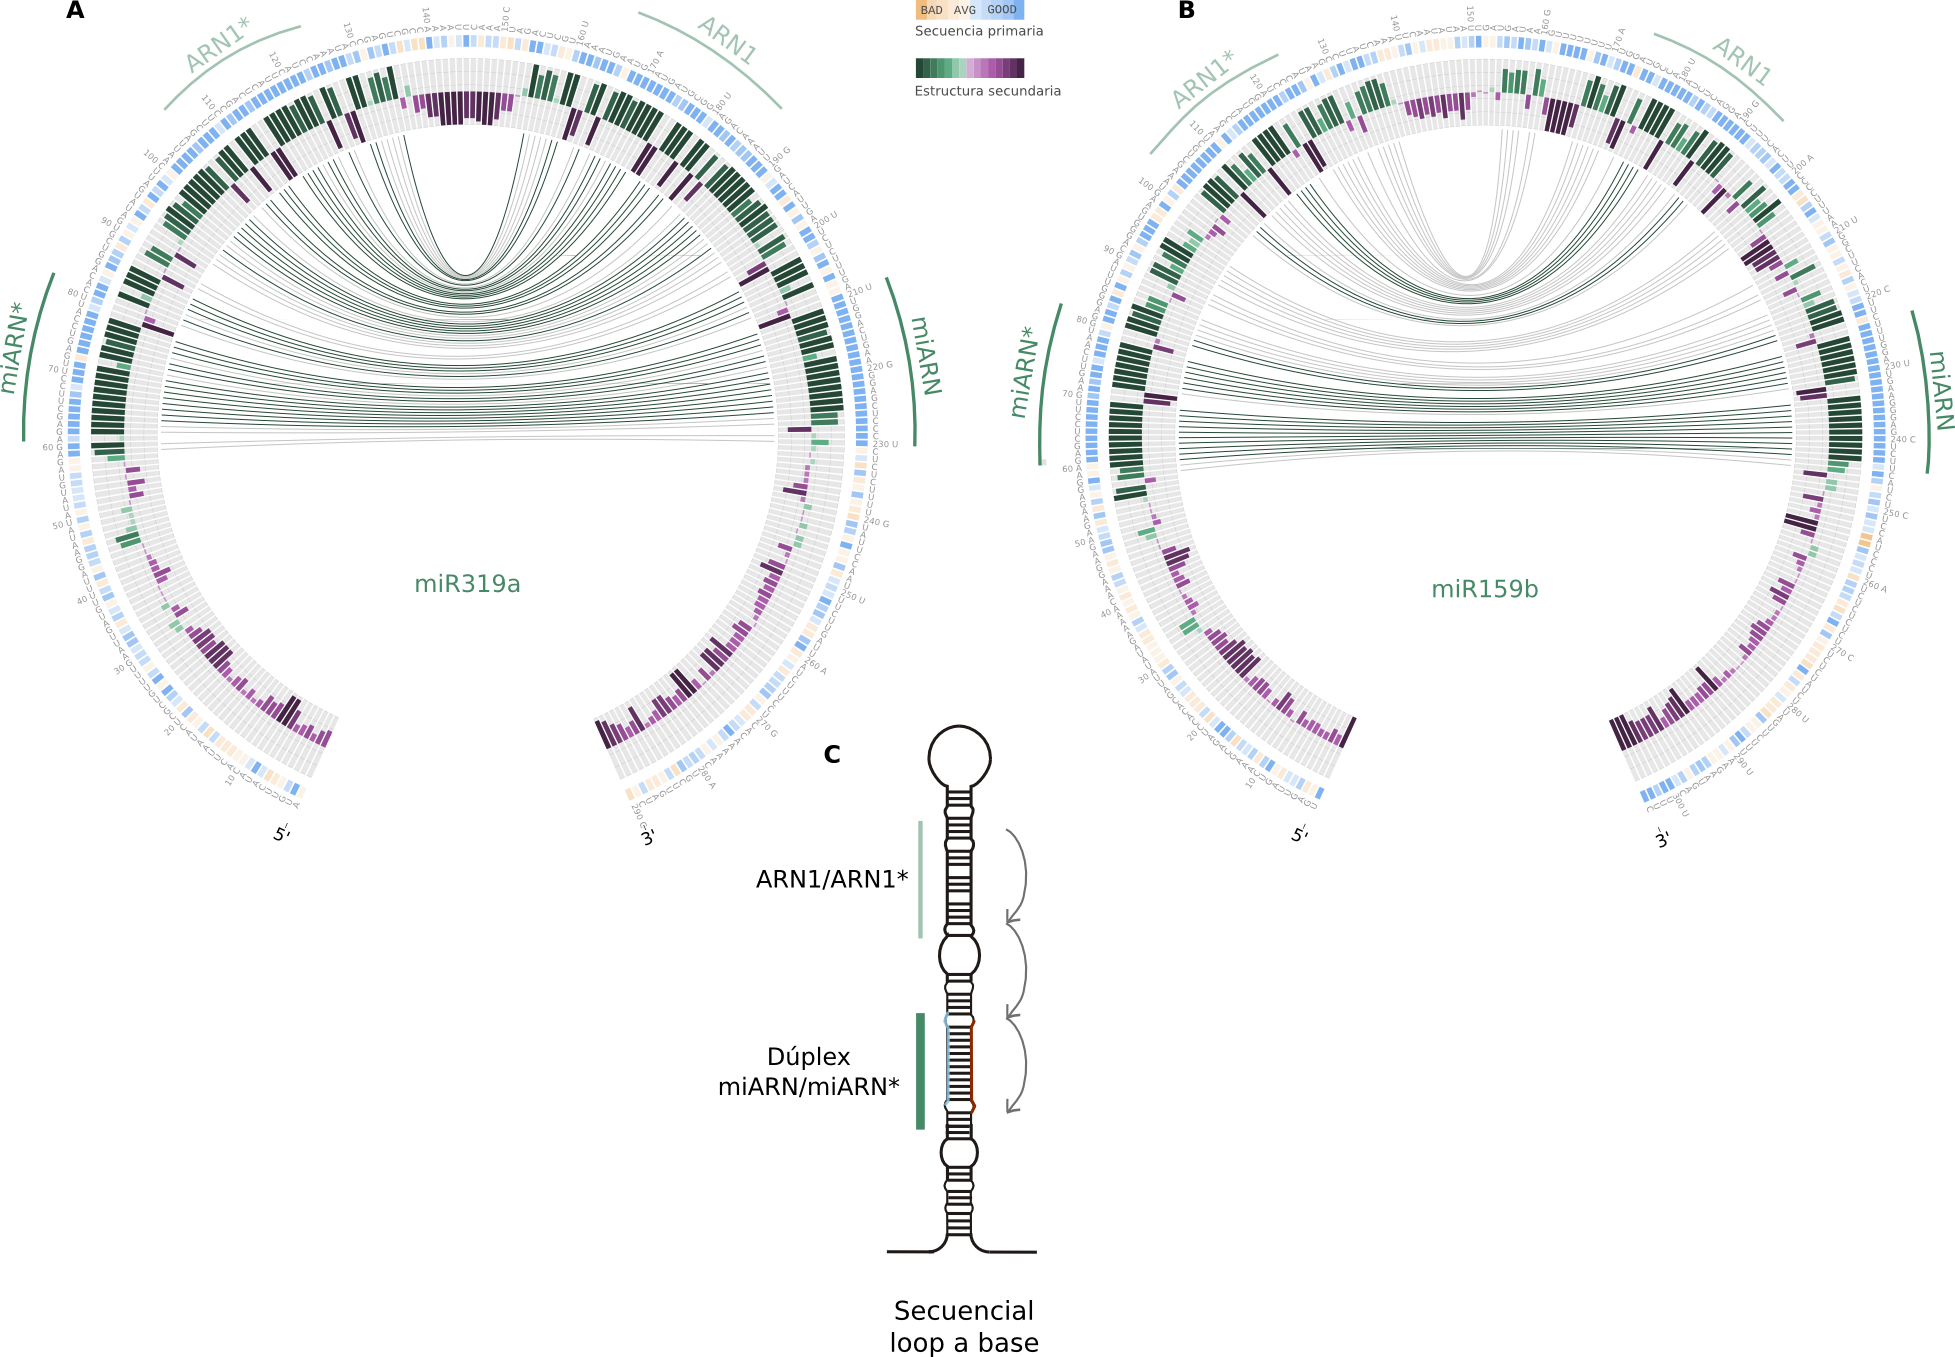
\includegraphics[width=1.4\textwidth]{seqLTB_circos.png}
        \caption[Circos de precursores con mecanismos de procesamientos secuenciales de loop a base]{
        \textbf{Circos de precursores con mecanismos de procesamientos secuenciales de loop a base}
		 \textbf{(A)} Circos del precursor del miR319a.
		 \textbf{(B)} Circos del precursor del miR159b.
		 \textbf{(C)} Estructura de precursores procesados secuenciales de loop a base.
		 En \textbf{(A)} y \textbf{(B)} se puede observar que los otros ARNs pequeños están conservados de la misma manera que el miARN y el miARN*.
        Con líneas verde fuera del Circos se muestra la región que corresponde al miARN y al miARN*. 
        Con líneas verde claro fuera del Circos se muestran otros ARN pequeños generados a partir del primer y segundo corte por DCL1.
		}
         \label{fig:seqLTB_circos}
    \end{figure}
\end{landscape}


\subsection{El tamaño del loop es muy variable en precursores que se procesan desde abajo.}

Una vez que hemos identificado los distintos precursores provenientes de estas 30 especies, decidimos hacer estudios adicionales sobre las dominios de los mismos.
Para cada precursor en distintas especies, realizamos una búsqueda de motivos conservados con la herramienta MEME \citep{pmid22115189} (Figura \ref{fig:miR160a_meme} y \ref{fig:miR172_meme}).
Hicimos esto para poder ver de manera visual cuáles eran los patrones comunes entre las distintas especies y donde se localizaban dentro del precursor.
La búsqueda se hizo sobre elementos conservados de 20-23 nucleótidos y los parámetros utilizados se detallan en Materiales y Métodos (sección \ref{sec:meme}).

De acuerdo a la literatura, esperabamos que los motivos más conservados dentro del precursor sean el miARN y el miARN*.
Si bien las secuencias que encontramos como las conservadas se superponían tanto con el miARN y el miARN*, en ocasiones observamos que estaban desfasada por uno o dos nucleótidos.
Nuestra interpretación es que es posible que el sitio de corte de DCL1, que se extiende por fuera de la secuencia del miARN y el miARN* tenga ciertos requisitos de estructura primaria y secundaria y de ahí su conservación.

Cuando visualizamos la localización de las secuencias conservadas en el contexto de los precursores que se procesan desde el loop observamos que las características del mismo estaban conservadas en las distintas especies.
Vemos que el precursor del miR160a el tamaño de la región que comprende al tallo superior y al loop está conservada en tamaño y varía entre 35-40 nt (Figura \ref{fig:miR160a_meme}).

Sin embargo cuando visualizamos los precursores que se procesan desde la base, pudimos observar que el tamaño de la región que comprende al tallo superior y al loop es muy variado en un mismo precursor en distintas especies.
Para el miR172a esta región puede variar entre 40nt hasta 115nt (Figura \ref{fig:miR172_meme}). 
Interpretamos que esta variación se debe a que los determinantes estructurales para su procesamiento están en la base del precursor, mientras que la estructura del loop es proclive a variaciones sin afectar el procesamiento del mismo.


\begin{landscape}
    \begin{figure}[htbp!] 
        \centering    
        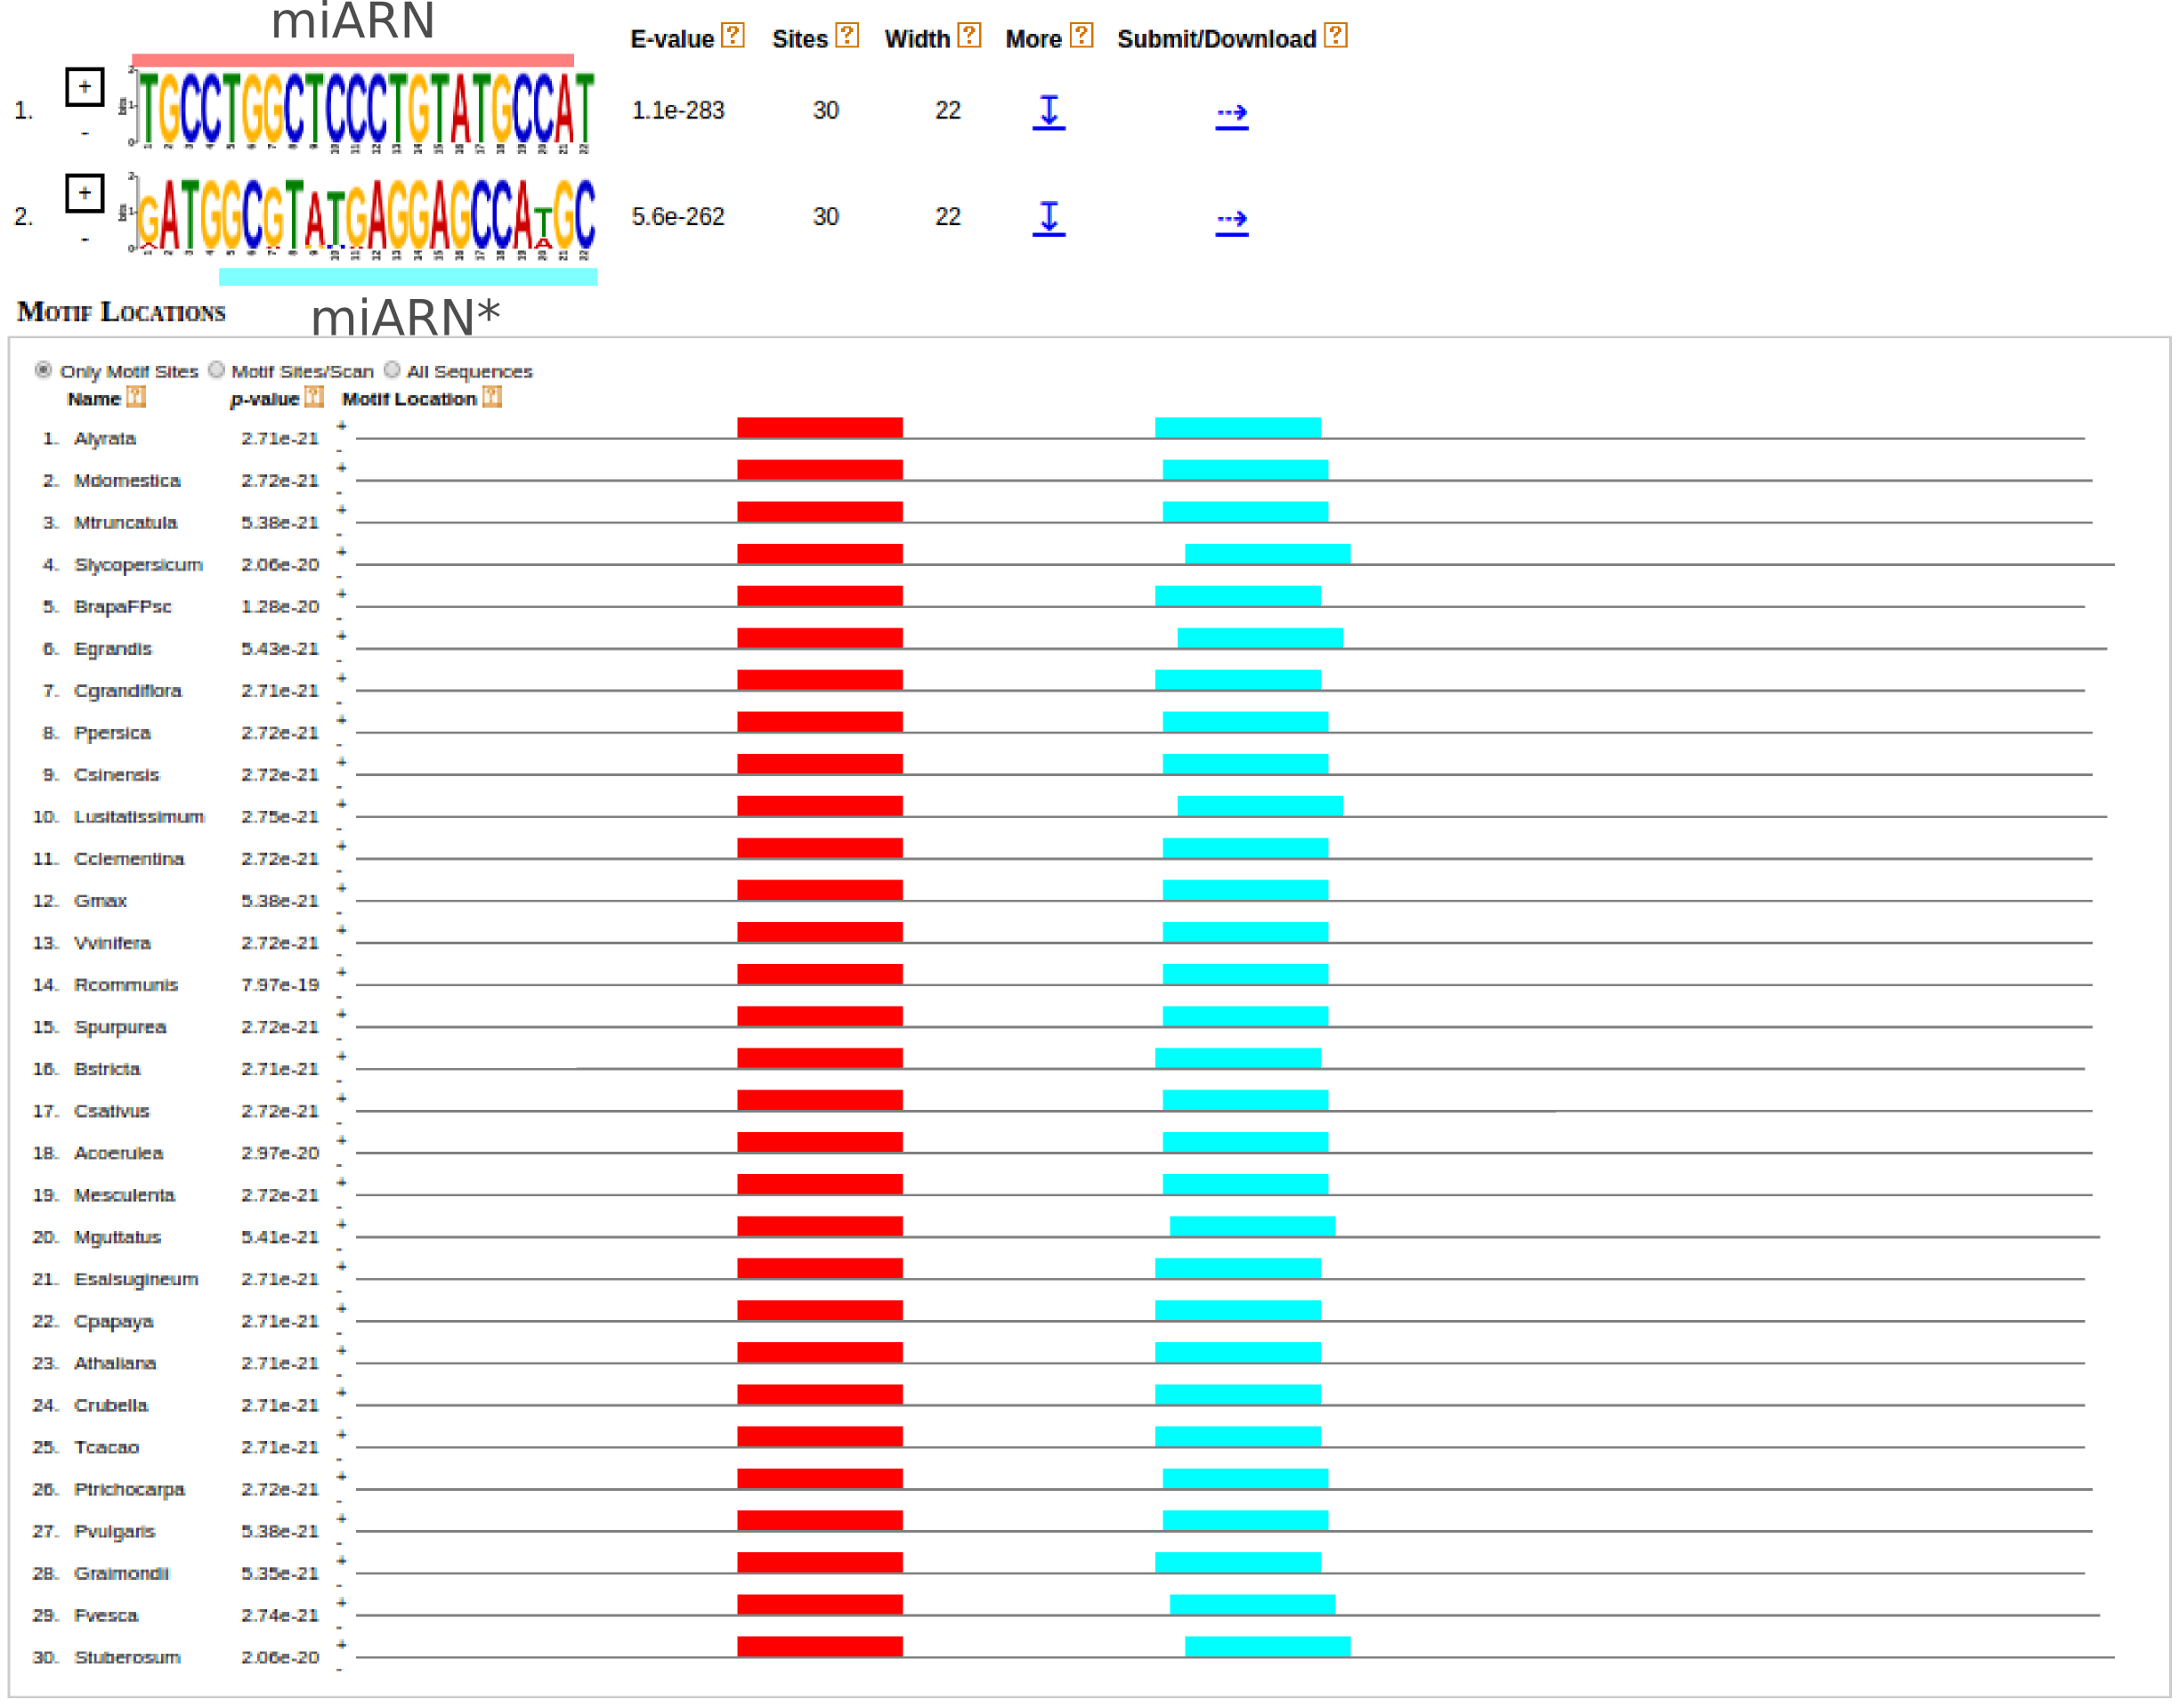
\includegraphics[width=1.3\textwidth]{miR160a_meme.png}
        \caption[Variacion del loop terminal en precursores miR172a]{
			\textbf{Variacion del loop terminal en precursores miR172a}
        Se muestra el MEME donde se pueden observar los motivos conservados dentro de los precursores del miR160a en distintas especies.
        En color rojo el primer motivo conservado comprende parte del miR160 (logo 1).
        El segundo motivo más conservado comprende parte del miR160* (logo 2).
        Se puede observar que la el tamaño de la región que comprende al tallo superior y al loop no varía en distintas especies.
        }
        \label{fig:miR160a_meme}
    \end{figure}
\end{landscape}

\begin{landscape}
    \begin{figure}[htbp!] 
        \centering    
        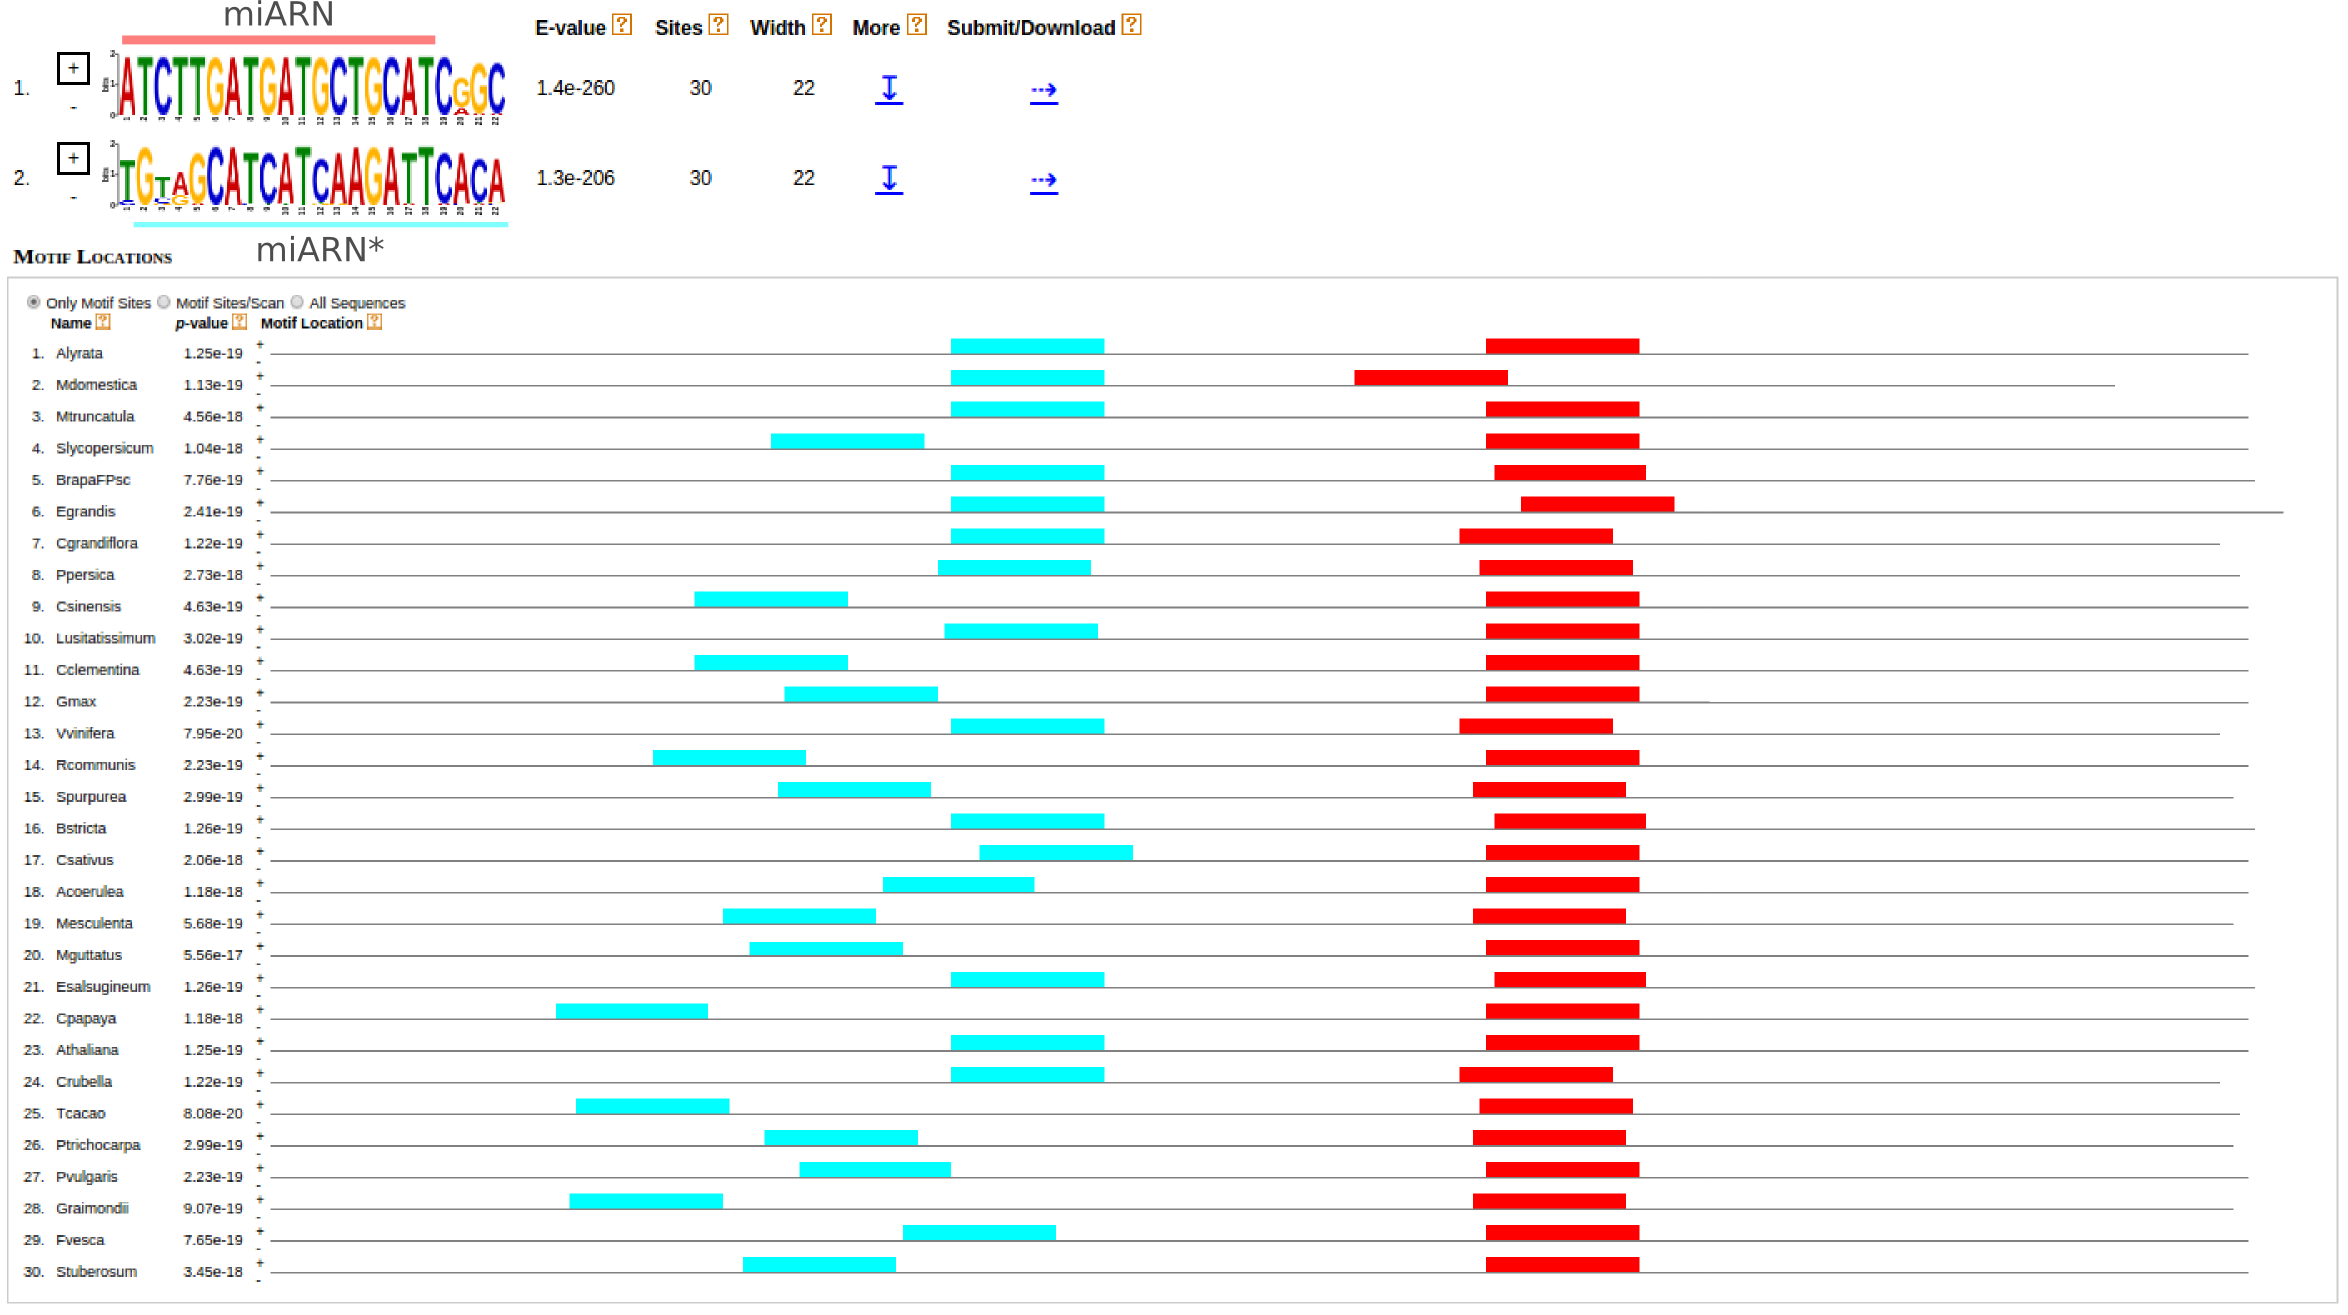
\includegraphics[width=1.4\textwidth]{miR172_meme.png}
        \caption[Variacion del loop terminal en precursores miR172a]{
			\textbf{Variacion del loop terminal en precursores miR172a}
        Se muestra el MEME donde se pueden observar los motivos conservados dentro de los precursores del miR172a en distintas especies.
        En color rojo el primer motivo conservado comprende parte del miR172 (logo 1).
        El segundo motivo más conservado comprende parte del miR172* (logo 2).
        Se puede observar que la el tamaño de la región que comprende al tallo superior y al loop es muy variado en distintas especies.
        }
        \label{fig:miR172_meme}
    \end{figure}
\end{landscape}


\subsection{Procesamiento mixto de miembros de la familia del miR170/miR171.}

En general, se considera que diferentes miembros de una misma familia de miARNs comparten la misma vía de biogenésis ya que se cree que las familias de miARNs se expanden por eventos de duplicación de un gen ancestral \citep{pmid15565108}.
Sin embargo, ciertos el procesamiento de miembros de ciertas familias pueden variar de uno a otro \citep{Bologna2013}.
Esto sucede, por ejemplo, en la familia del miR171 donde en \textit{A. thaliana} existen tres miembros. 
El precursor del miR171a es procesado de base a loop, mientras que los precursores del miR171b y miR171c son procesados de loop a base.

Nos pusimos a analizar esta familia en detalle para ver si los patrones de conservación y estructura secundaria eran similares o diferentes (Figura \ref{fig:familia_miR171_circos}).
Observamos que el miR171a, que es procesado corto de base a loop, tiene un patrón de conservación similar a los precursores procesados de base a loop, donde el tallo inferior es estructurado y conservado, como era de esperarse (Figura \ref{fig:familia_miR171_circos} B).
Por el contrario, el miR171c, que es procesado corto de loop a base, muestra conservación en el tallo superior, que además es estructurado, y no así el tallo inferior (Figura\ref{fig:familia_miR171_circos} A).


Esta familia mixta, presenta dos patrones claros y diferentes de conservación de secuencia primaria y de estructura secundaria.
Demostrando que este análisis es sensible a la selección de ortólogos para miembros de una misma familia.
Donde para el Circos del precursor del miR171a se incluyen 24 especies y para el Circos del precursor del miR171c se incluyen las 30 especies estudiadas.

\begin{landscape}
    \begin{figure}[htbp!] 
        \centering    
        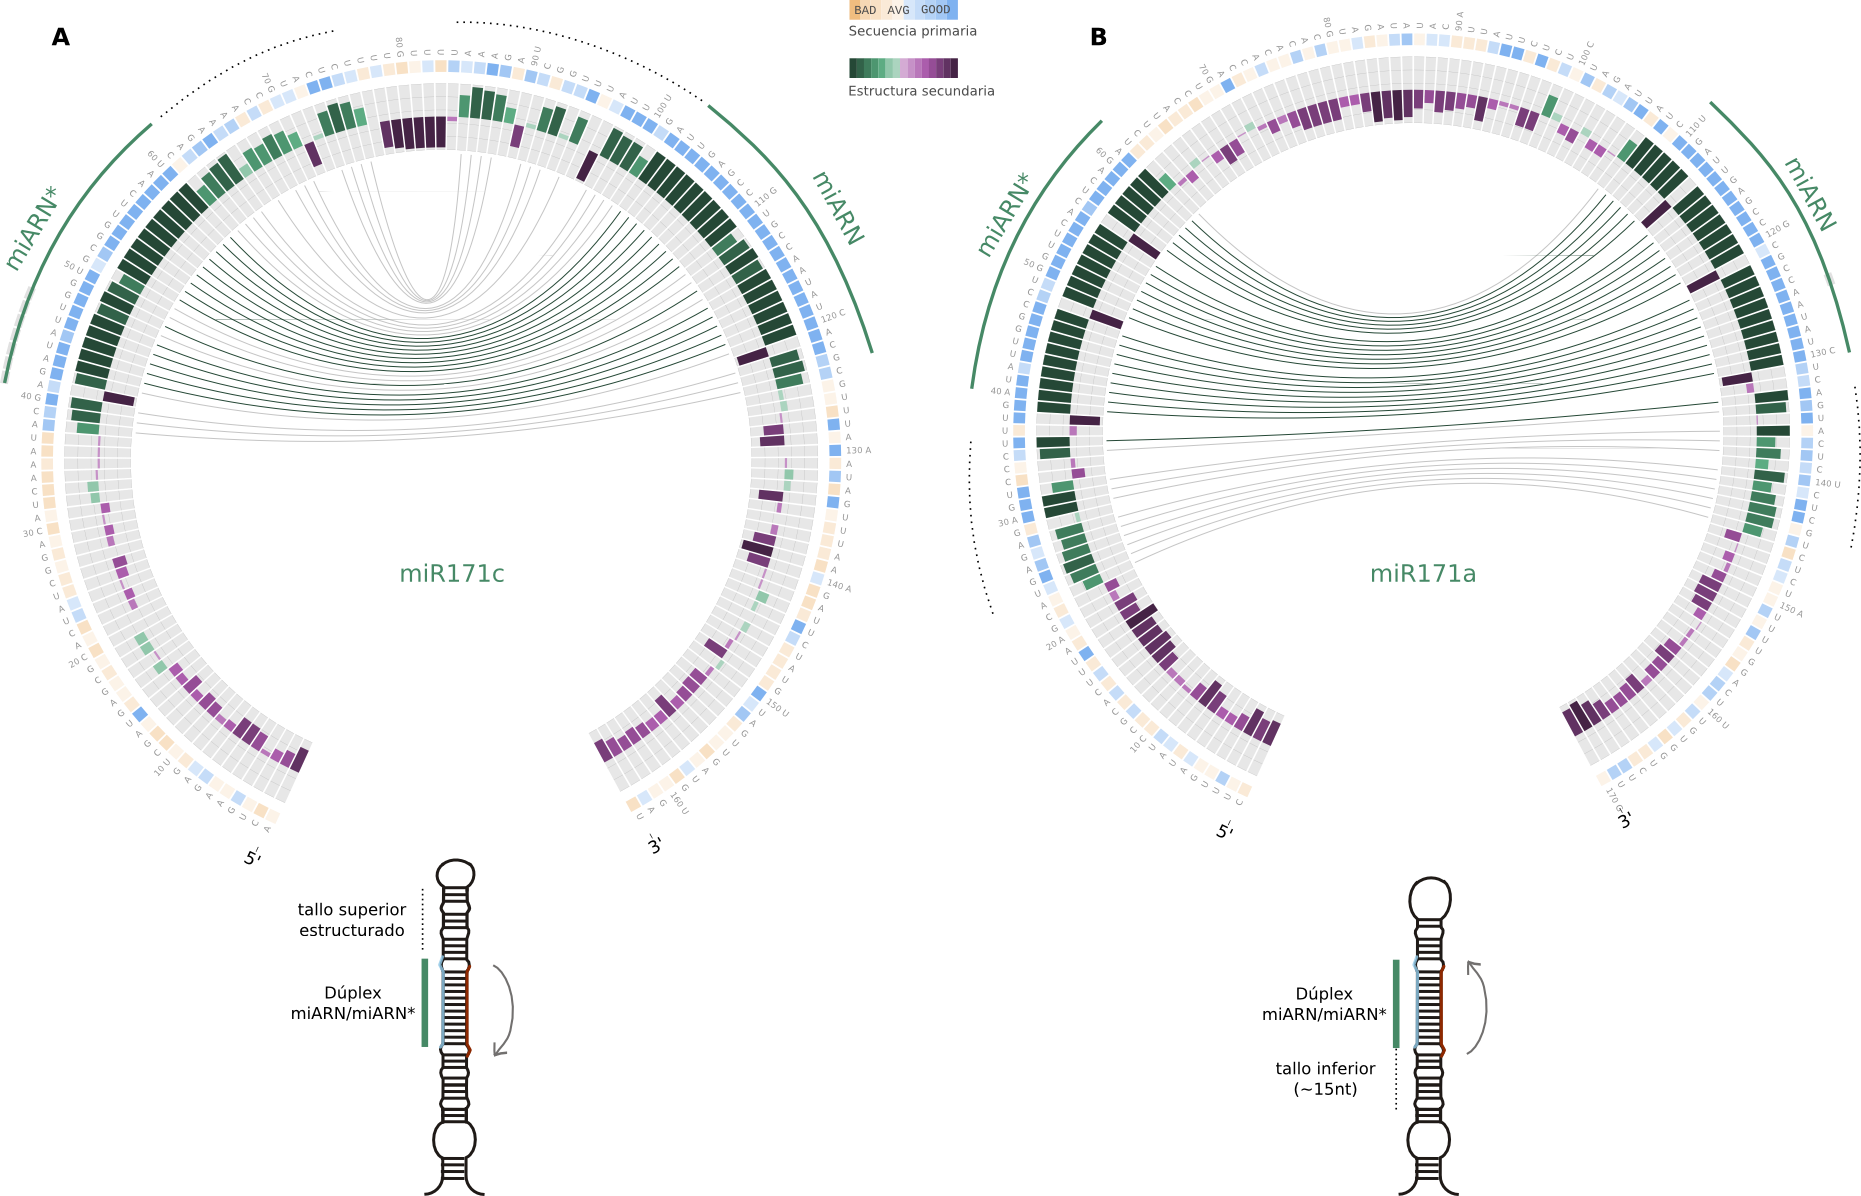
\includegraphics[width=1.4\textwidth]{familia_miR171_circos.png}
        \caption[Patrón de conservación de la familia con procesamiento mixto del miR170/miR171]{
        \textbf{Patrón de conservación de la familia con procesamiento mixto del miR170/miR171}
		 \textbf{(A)} Circos del precursor del miR171c que es procesado de loop a base.
		 \textbf{(B)} Circos del precursor del miR171a que es procesado de base a loop.
            Se puede observar que el miR171c, que es procesado corto de loop a base, muestra conservación en el tallo superior.
            Por el contrario el miR171a, que es procesado corto de base a loop, el tallo inferior es estructurado y conservado
			Con líneas de puntos se muestra fuera del Circos la región que corresponde en \textbf{(A)} al tallo superior y en \textbf{(B)} al tallo inferior de $\sim$15nt.
            Además, se muestra un esquema del mecanismo de procesamiento correspondiente a cada precursor.
			}
         \label{fig:familia_miR171_circos}
    \end{figure}
\end{landscape}


\subsection{Visualización por Circos de precursores con mutaciones puntuales que afectan el procesamiento de miARNs en plantas.}

Se ha demostrado recientemente que un polimorfismo de origen natural que ocurre en el gen del miR164a afecta a la forma de la hoja y la arquitectura del vástago en \textit{A. thaliana}, debido a una mutacion presente en ecotipo C24, con los efectos de ser modificados por loci adicionales en el genoma \citep{pmid22206705}.
Una sustitución única en un par de bases en la secuencia complementaria del miARN altera la estabilidad predicha del dúplex miARN/miARN*.
Se reduce con ello, en gran medida, la acumulación del miARN maduro, probablemente porque interfiere en el procesamiento del precursor.
Además, se demostró en ese mismo artículo que no es una rara excepción y que las cepas naturales de \textit{A. thaliana} albergan decenas de polimorfismos similares que afectan al procesamiento de una amplia gama de precursores de miARNs.

A nivel de secuencia los alelos de Col-0 y C24 son diferentes sólo por un par de polimorfismos simples.
Uno de ellos afecta a una C en el miARN* que aparea con una G en la posición dos del miARN (nos referimos a esta posición como *2) (Figura \ref{fig:miR164_ss_bp} A).

\begin{figure}[htbp!] 
	\centering    
	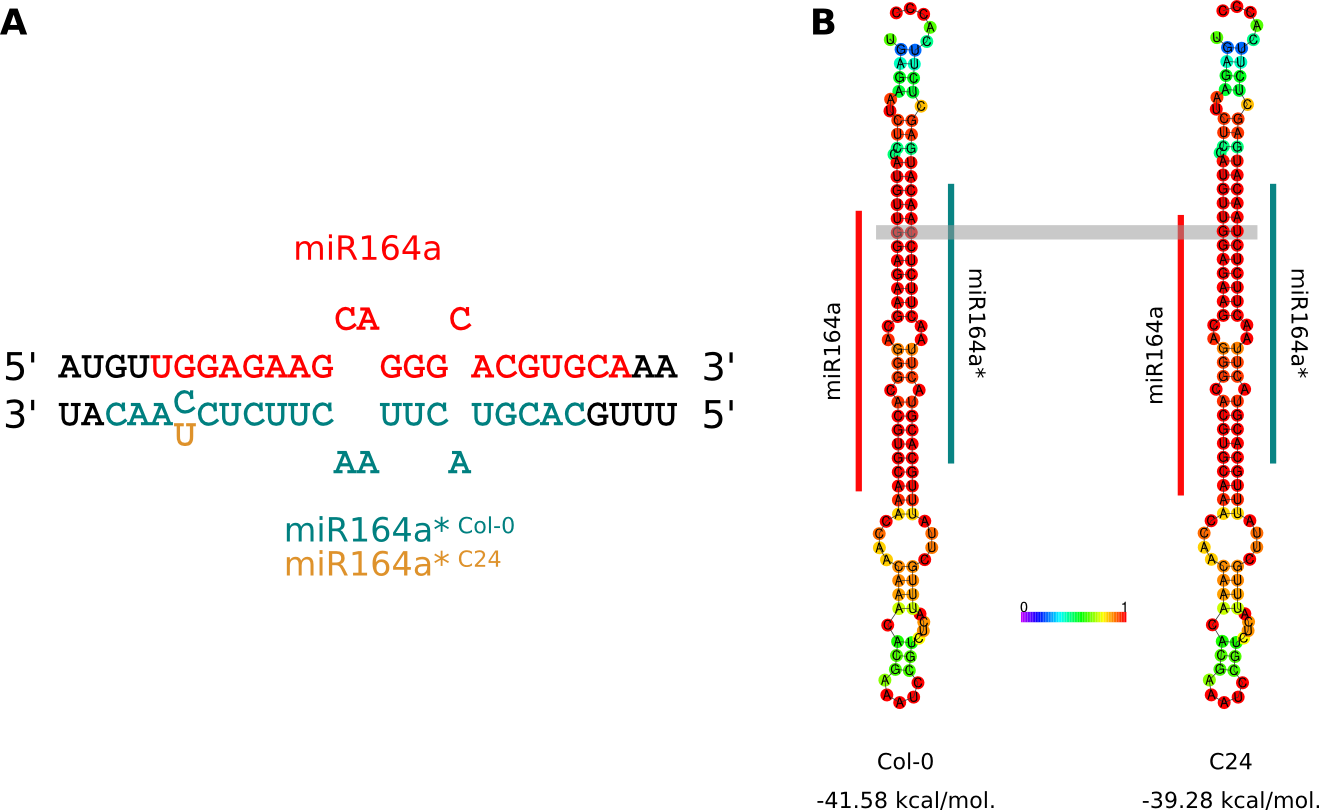
\includegraphics[width=0.8\textwidth]{miR164_ss_bp.png}
	\caption[Dúplex del miR164a/miR164a* y estructura secundaria del precursor]{
		\textbf{Dúplex del miR164a/miR164a* y estructura secundaria del precursor.}
		\textbf{(A)}. Se muestra el apareamiento de bases en el precursor del miR164a.
		El miARN se muestra en rojo y el miARN* en azul.
		En la posición *2, el alelo alternativo C24 se muestra en naranja.
		\textbf{(B)}. Se muestra la estructura secundaria predicha del precursor del miR164a.
		La barra gris horizontal indica el polimorfismo, un G:C en Col-0 y un G:U en C24.
		Los colores indican probabilidad de pares de bases.
	}
	\label{fig:miR164_ss_bp}
\end{figure}

Se puede ver que el remplazo de una G:C en el miR164$a^{Col-0}$ por un par no canónico G:U en el miR164$a^{C24}$, incrementa ligeramente la energía libre del plegado del precursor que cambia de -41.58 kcal/mol a -39.28 kcal/mol.
Pero se observa que no se modifica la estructura secundaria del miR164a si aceptamos que el par canónico G:U se forme en esta región (Figura \ref{fig:miR164_ss_bp} B). 

Realizamos el Circos del miR164a en distintas especies para ver como era la conservación de la base en la posición 2* que hace que el precursor no pueda ser procesado de manera correcta.
Lo que pudimos observar es que dicha posición del miR164a* está conservada en dicotiledóneas y se mantiene sin cambios en todas las especies (Figura \ref{fig:miR164a_circos}).
Además esa base está siempre apareada con la base correspondiente del miARN maduro, formando un G:C (Figura \ref{fig:miR164a_circos}).

También se puede observar que en la secuencia del miR164a* existen mutaciones en distintas bases en distintas especies, pero no en la base que estamos estudiando.
Esto sugiere que esa base en particular es importante para la estabilidad del precursor y su buen procesamiento.

\begin{figure}[htbp!] 
    \centering    
    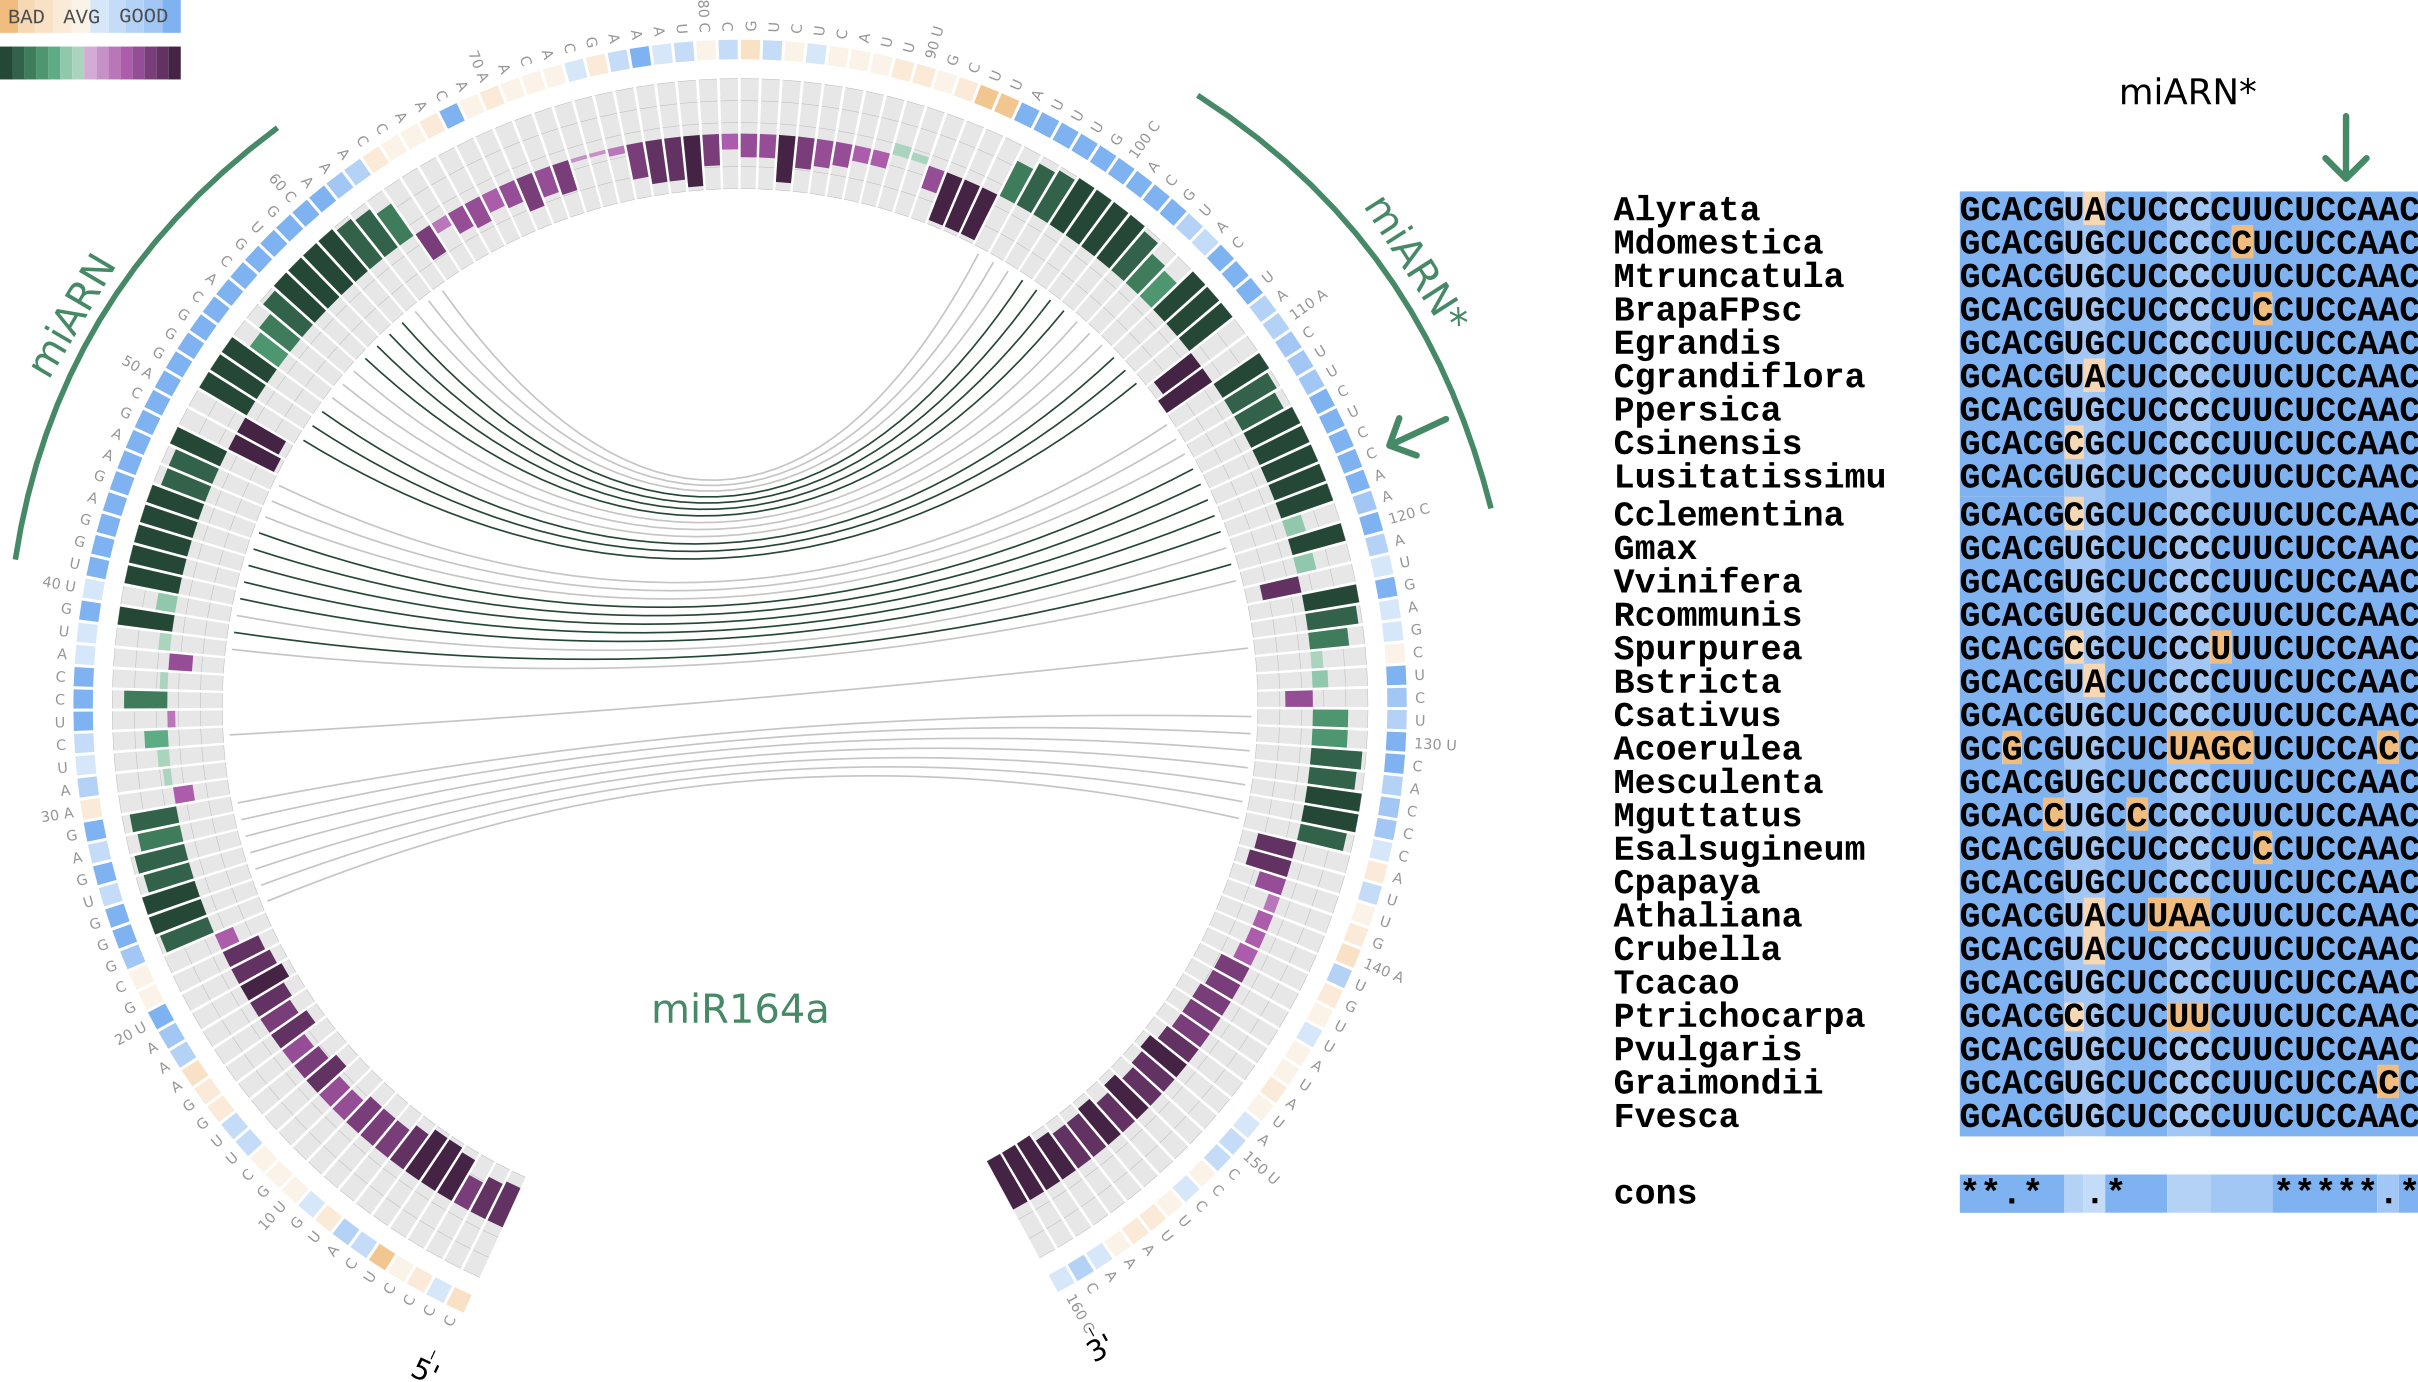
\includegraphics[width=1\textwidth]{miR164a_circos.png}
    \caption[Circos del miR164a]{
        \textbf{Circos del miR164a}.
        \textbf{(A)} Se representa el Circos del miR164a.
        \textbf{(B)} Se representa El alineamiento del miR164a en distintas especies. 
        Con una flecha naranja se destaca la posición *2 a estudiar, en el Circos y en el alineamiento.
    }
    \label{fig:miR164a_circos}
\end{figure}

\begin{figure}[htbp!] 
	\centering    
	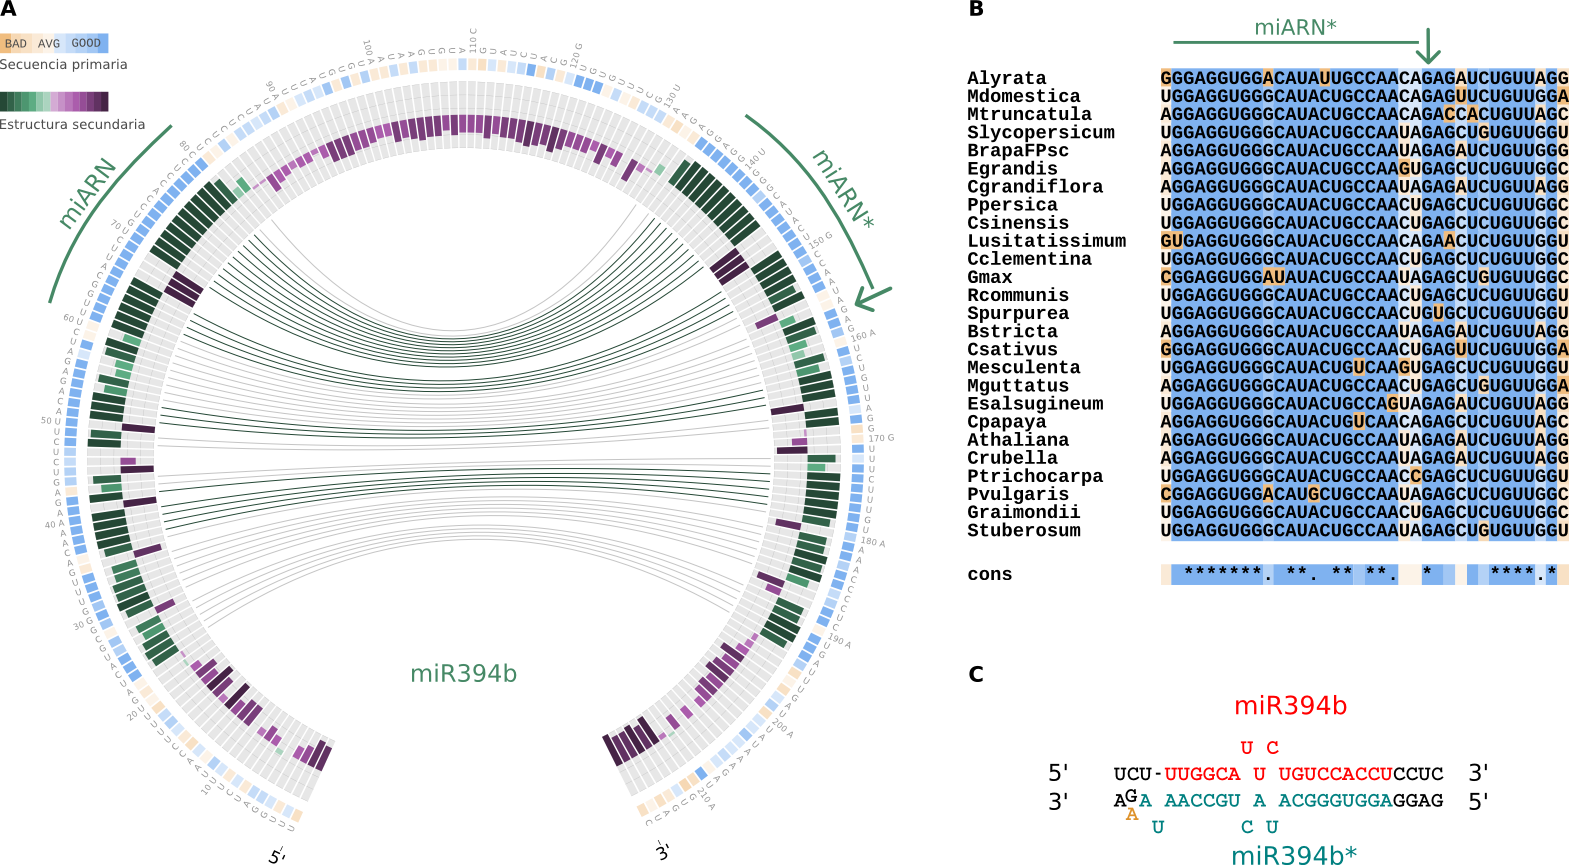
\includegraphics[width=1\textwidth]{miR394b_circos_aliniamientos.png}
	\caption[Patrón de conservación del precursor del miR394b]{
		\textbf{Patrón de conservación del precursor del miR394b}.
		\textbf{(A)} Se muestra el Circos del miR394b.
		\textbf{(B)} Se muestra el alineamiento del miR394b en distintas especies. 
		Con una flecha naranja se destaca la posición a estudiar, en el Circos y en el alineamiento.
		\textbf{(C)} Apareamiento de bases en el precursor del miR394b.
		El miARN se muestra en rojo y el miARN* en azul.
		En naranja se muestra la posición de la mutación G por A en el tallo inferior del precursor del mir394b-1.
		
	}
	\label{fig:miR394b_circos_aliniamientos}
\end{figure}

En otro trabajo, se estudió un alelo mutante del miR394b, llamado mir394b-1, que tiene un ``mismatch'' en el tallo inferior del precursor del miR394b \citep{pmid23333352}.
La mutante incrementa dramáticamente la terminación del meristema apical.   
En la figura \ref{fig:miR394b_circos_aliniamientos} C, se muestra el apareamiento de bases en el precursor del mir394b y mir394b-1, donde el miARN se muestra en rojo y el miARN* en azul.
Y en naranja se muestra la posición de la mutación del precursor del mir394b-1 donde la G es reemplazada por una A con respecto al mir394b.
En este caso se mostró que los niveles de maduro en el precursor del mir394b-1 se ven fuertemente disminuidos aunque no completamente ausentes \citep{pmid23333352}. 

Para varios precursores de plantas hemos visto anteriormente que esa región que corresponde al tallo inferior es crucial para su procesamiento.
En este caso mostramos el Circos correspondiente al miR394b, para poder visualizar que es lo que sucede con esta mutación puntual fuera del dúplex miARN/miARN* (Figura \ref{fig:miR394b_circos_aliniamientos}).
Vemos, como en el caso del miR164a, esta mutación que afecta al procesamiento del precursor y a la acumulación del miARN maduro, está conservada en todas las especies estudiadas.
Esto sugiere que esta base es importante para el procesamiento y que no sólo mutaciones de una base dentro del dúplex miARN/miARN* pueden afectar el procesamiento, sino que mutaciones simples en el precursor puede afectar el reconocimiento de DCL1. 


La metodología empleada y la visualización por medio de los Circos permite deducir cuales son las bases o apareamientos conservados en distintas especies.
Pensamos además que estas bases son importantes por se para el procesamiento del precursor y la liberación del miARN maduro , ya que puede observarse una correlacion entre la conservación y las mutaciones puntuales descriptas.
Esta información también podría ser utilizada para ayudar en el diseño de miARNs artificiales en distintas especies y aumentar su eficiencia.

\subsection{Visualización por Circos de precursores de plantas conservados en monocotiledóneas.}

Se conocen muchas familias de precursores conservados en plantas, algunos de ellos conservados desde musgos hasta dicotiledóneas \citep{pmid15849273,Axtell2008343,citeulike:8816489}.
Si bien la mayoría de los precursores de plantas utilizados hasta esta parte del trabajo están conservados en dicotiledóneas y monocotiledóneas, muchos fueron evolucionando encontrandose nuevos miembros de algunas familias en especies más recientes y perdiendose otros.    
Es por esto que separamos a los precursores de plantas en dicotiledóneas y monocotiledóneas, y en esta parte del trabajo nos enfocamos en estas últimas.
Las especies utilizadas de monocotiledóneas se pueden ver en la Figura \ref{fig:treePhytozome} de Materiales y Métodos.

Existe una variante del miR396 que fue detectada por primera vez en arroz \citep{pmid15805478} y estudios posteriores indicaron que la misma es especifica de monocotiledóneas \citep{pmid18416839, pmid19936050}.
El sitio complementario al miR396 de los GRFs (genes blanco del miR396) en dicotiledóneas posee un nucleótido, que en el apareamiento entre el miARN y el ARNm genera un bulge.
Es muy interesante que la G extra (entre la posición 7-8 del miARN) presente en la variante de monocotiledóneas elimina este bulge en el apareamiento con el sitio blanco de los GRFs.

Realizamos el gráfico del Circos del miR396e de Arroz, donde pudimos detectar ortólogos en todas las plantas monocotiledóneas estudiadas en nuestro trabajo (Figura \ref{fig:circos_monocots_miR396e}).
Observamos que el nucleótido extra, que le da identidad a la variante de monocotiledóneas, está conservado en todas las especies.
Se observa que a nivel de secuencia primaria el precursor está conservado, pero el patrón de conservación no coincide exactamente con los patrones de conservación vistos anteriormente para los precursores que se procesan desde la base como los que se procesan desde el loop.
En particular se observa conservación de secuencia primaria y secundaria por arriba y por debajo del dúplex (Figura \ref{fig:circos_monocots_miR396e}).

Este análasis en monocotiledóneas, demuestra que el enfoque bioinformático para el estudio de la evolución de precursores de miARNs en plantas también puede ser utilizado para encontrar determinantes estructurales en un grupo de especies cercanas evolutivamente.  
Además, el mismo permite poder comparar patrones de evolución en distintos grupos de especies.

\begin{figure}[htbp!] 
    \centering    
    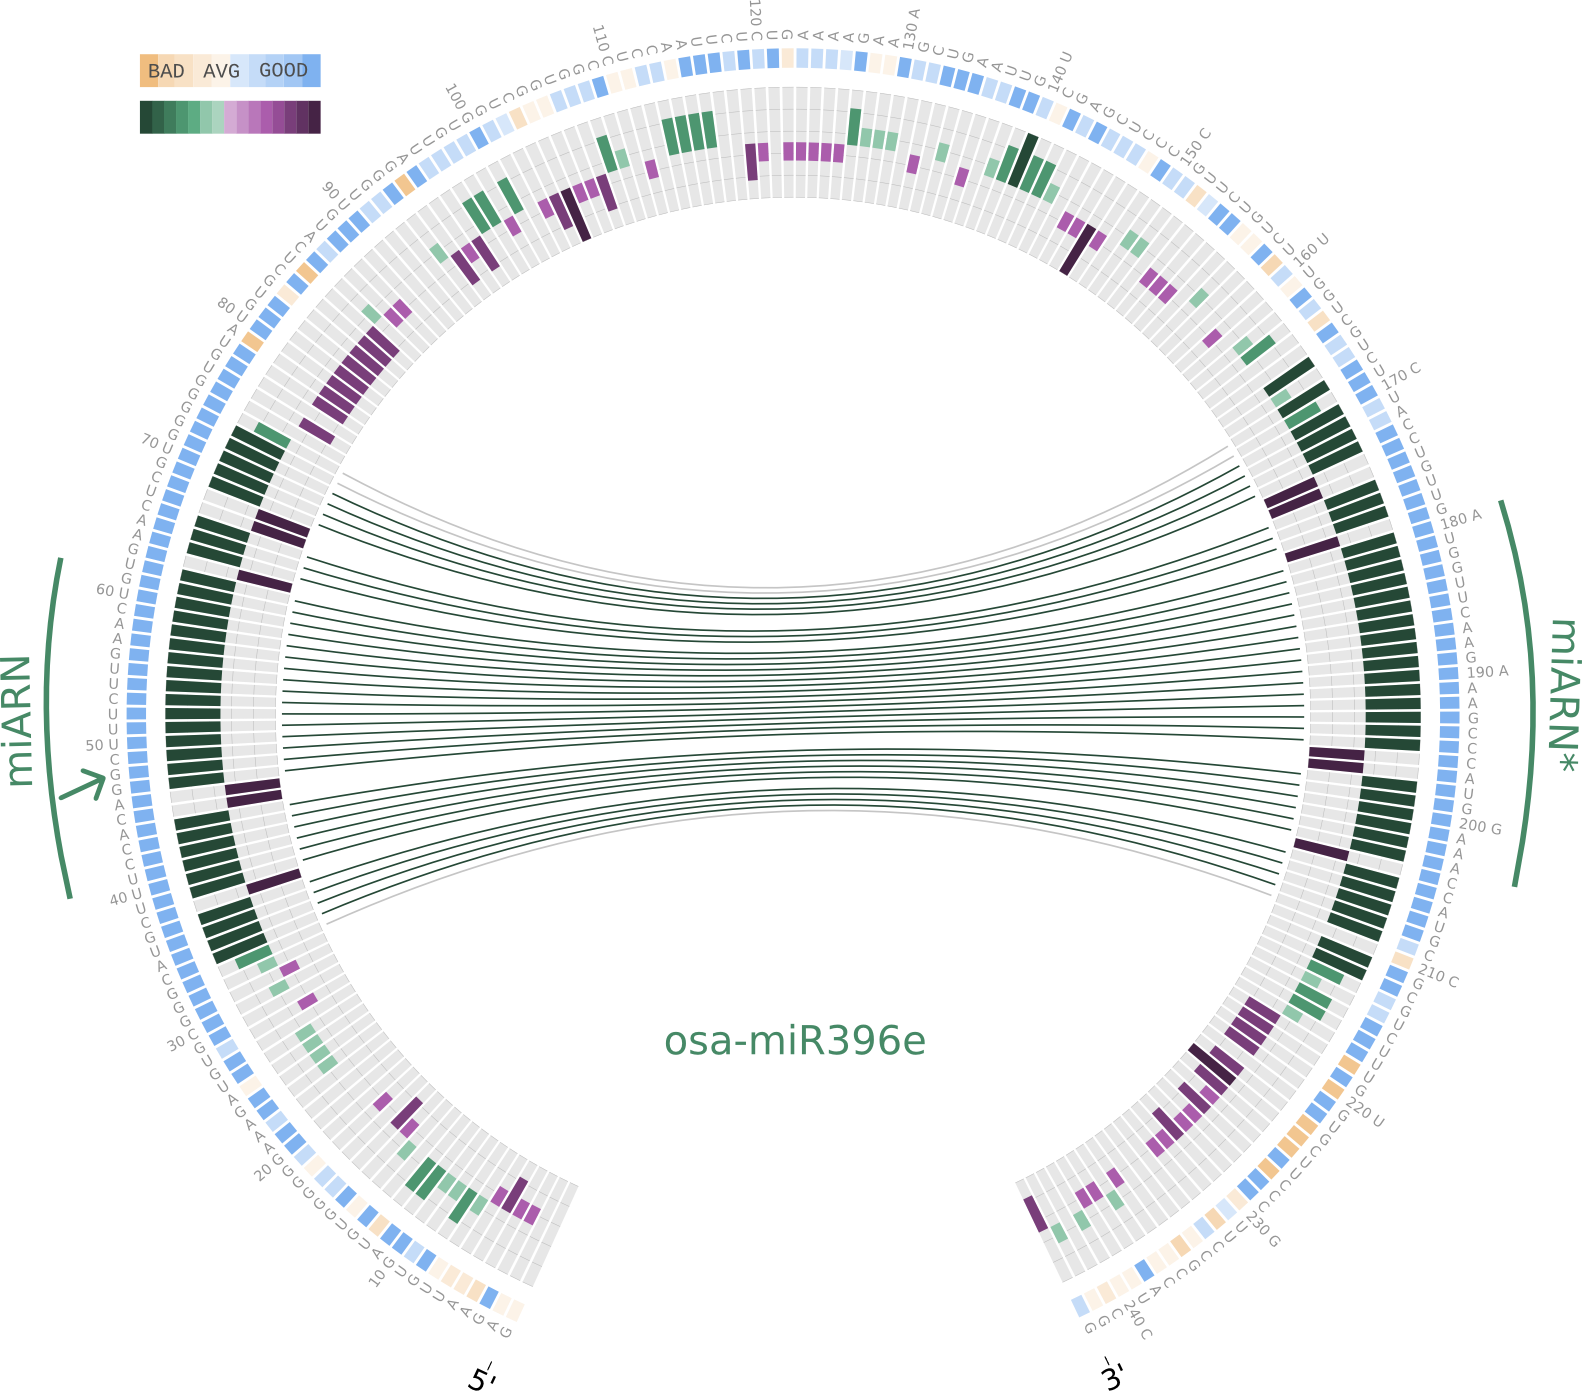
\includegraphics[width=1\textwidth]{circos_monocots_miR396e.png}
    \caption[Circos del miR172a]{
    \textbf{Circos del miR396e de monocotiledóneas}
    Se puede observar que el nucleótido extra, que le da identidad a la variante de monocotiledóneas, está conservado en todas las especies.
    Este nucleótido extra que se marca con una flecha naranja.
    }
     \label{fig:circos_monocots_miR396e}
\end{figure}

\subsection{Estrategia bioinformática para estudiar precursores de miARNs en animales.}

En animales existe un gran número de miARNs que están conservados en un gran rango de especies, incluso se han encontrado algunos miARNs conservados en humanos hasta gustanos \citep{pmid11081512}.
Si bien los miARNs en plantas y en animales comparten componentes básicos, su biogénesis y su modo de acción es diferente.
Una de las grandes diferencias con las plantas radica en que en animales el procesamiento de los precursores ocurre en dos pasos separados
en tiempo y espacio (Figura \ref{fig:procesamiento_animales}), mientras que en plantas ocurre íntegramente en el núcleo (Figura \ref{fig:biogenesis_accion}).

Además de las diferencias en la biogénesis, otra de las grandes diferencias entre plantas y animales consiste en las estructuras de los precursores de miARNs.
Los precursores de animales se caracterizan por presentar una estructura relativamente homogénea, que consta de un tallo imperfecto de una longitud de $\sim$65 nt, flanqueado por dos regiones desapareadas.
Estas dos regiones son un bucle terminal en un extremo y ARNsh en el otro.
En animales, la especificidad en la selección de la secuencia del miARN dentro del precursor está dada por el primer corte realizado por el complejo microprocesador.
Por otro lado, los precursores de miARNs de plantas presentan tamaños que varían desde los 50 a 900 nt, lo que se traduce en un amplio abanico de estructuras diferentes.

Para esta parte del trabajo de Tesis, utilizamos genomas de especies de \textit{Metazoa} entre ellos humano, mono, sapo, vaca y pez (Tabla \ref{table:db_metazoa}) y estudiamos que sucede con los precursores de miARNs conservados en animales.
Para esto partimos de los precursores de humanos definidos en miRBase y realizamos la búsqueda de ortólogos en otras especies al igual que lo hicimos en plantas.

\begin{table}[!htbp]
\centering
\small
\caption{Especies de \textit{Metazoa} utilizadas}
\label{table:db_metazoa}
\begin{tabular}{c}
\textbf{Animales}        \\
	Bos taurus               \\
	Canis familiaris         \\
	Equus caballus           \\
	Gallus gallus            \\
	Gorilla gorilla          \\
	Homo sapiens             \\
	Macaca mulatta           \\
	Monodelphis domestica    \\
	Mus musculus             \\
	Ornithorhynchus anatinus \\
	Petromyzon marinus       \\
	Sus scrofa               \\
	Xenopus tropicalis      
\end{tabular}
\end{table}

En la Figura \ref{fig:hsa-let-7a-1_circos} se muestra el Circos del precursor del miARN hsa-let-7a-1, un miembro de la familia let-7.
El precursor del miARN let-7 identificado en un estudio en \textit{C. elegans} fue uno de los primeros miARNs en ser descubiertos.
Actualmente ha sido predicho y validado en un gran número de especies.

En un artículo publicado en Nat. Struct. Mol. Biol., se encontró una ribonucleoproteína (hnRNP A1) que actúa como regulador negativo de let-7-a \citep{pmid20639884}.
HnRNP A1 se une al loop terminal del precursor de let-7-a e inhibe su procesamiento por Drosha.
En el Circos se puede observar que este loop terminal está conservado en las especies utilizadas (\ref{fig:hsa-let-7a-1_circos}).

\begin{figure}[htbp!] 
	\centering    
	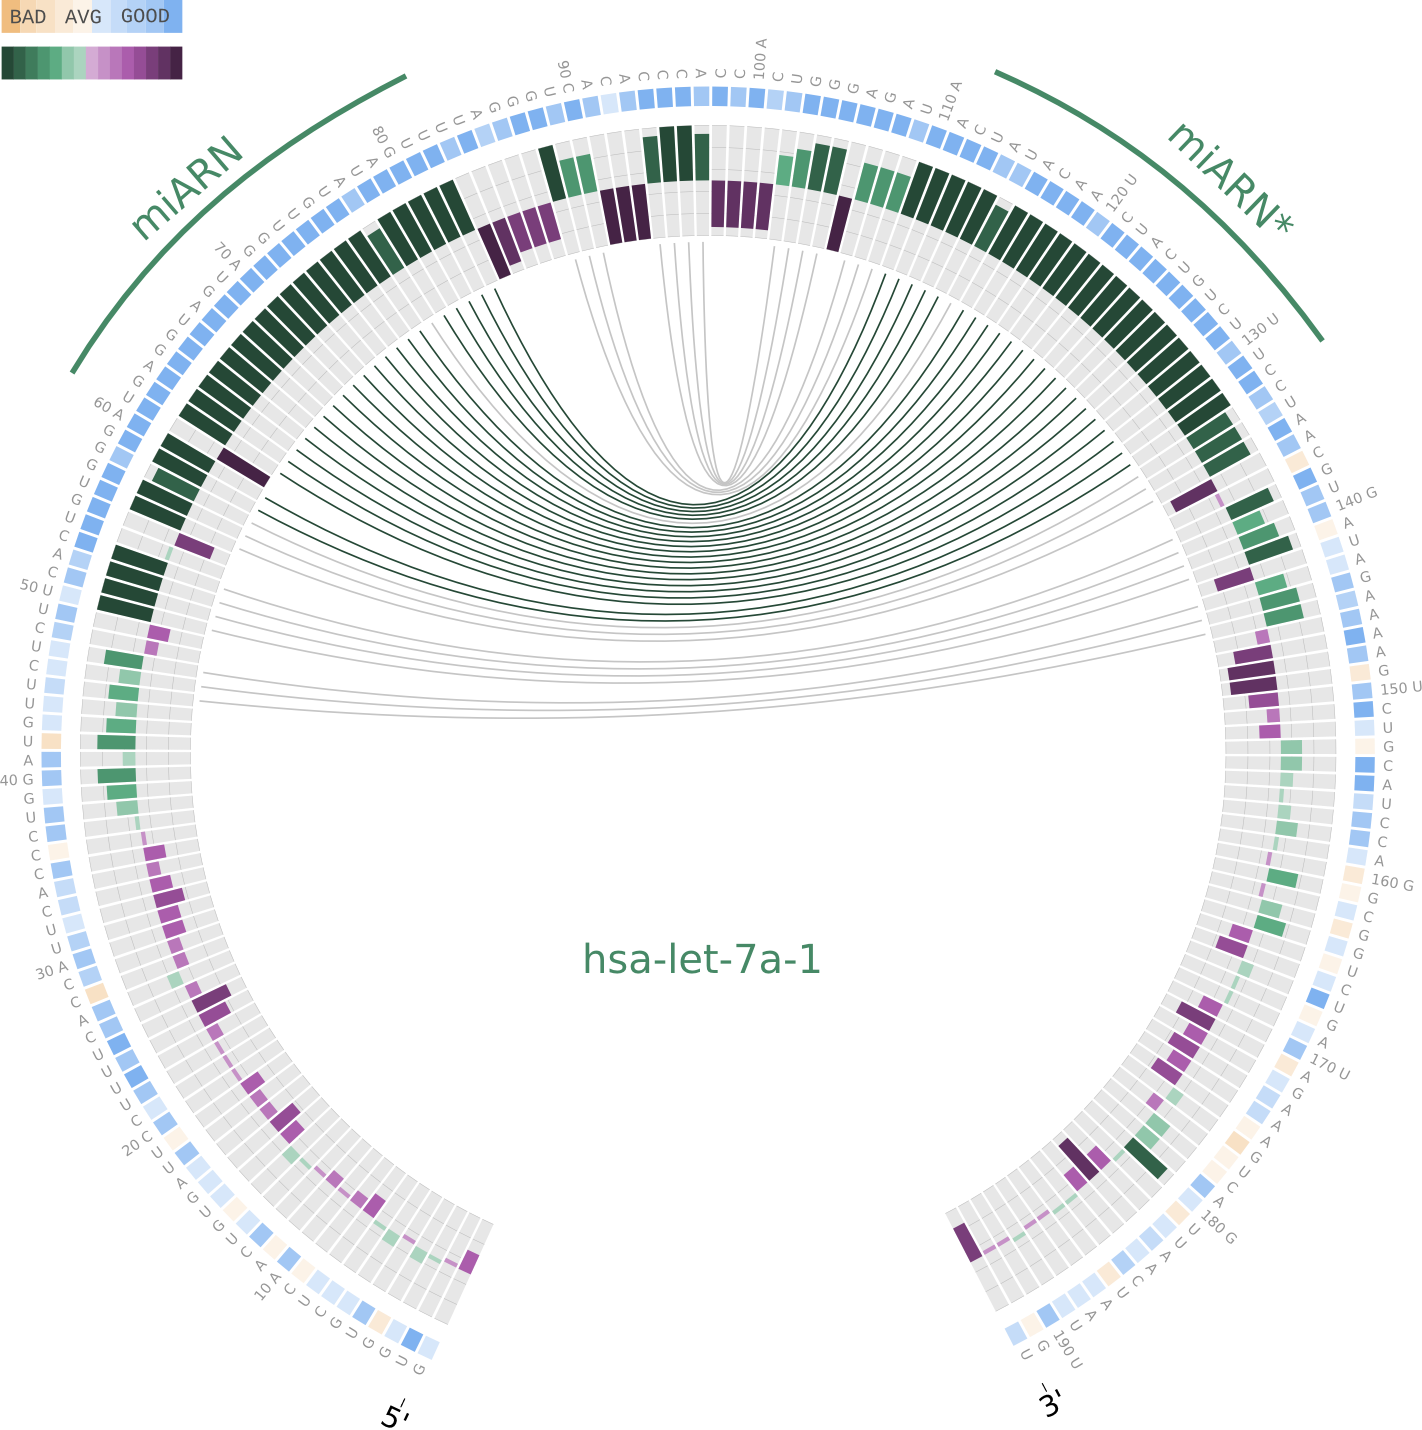
\includegraphics[width=1\textwidth]{hsa-let-7a-1_circos.png}
	\caption[Patrón de conservación del precursor del precursor del miARN hsa-let-7a-1]{
		\textbf{Patrón de conservación del precursor del precursor del miARN}.
	}
	\label{fig:hsa-let-7a-1_circos}
    Se puede observar que loop terminal (marcado en línea de puntos) está conservado en las especies utilizadas.
\end{figure}

La variación de los precursores de miARNs de plantas se debe en gran parte a la variación en el tamaño del loop.
Observamos el tamaño del loop terminal en precursores de plantas procesados cortos de base a loop o de loop a base y lo comparamos con el tamaño del loop terminal en precursores conservados en animales.
Se puede notar que el tamaño del loop en los precursores de plantas cortos de base a loop son más variables además de más grande.
En cambio el tamaño del loop terminal de los precursores de humano son pequeños y similares al tamaño del loop terminal de precursores de plantas loop a base.

%~ \begin{figure}[htbp!] 
	%~ \centering    
	%~ 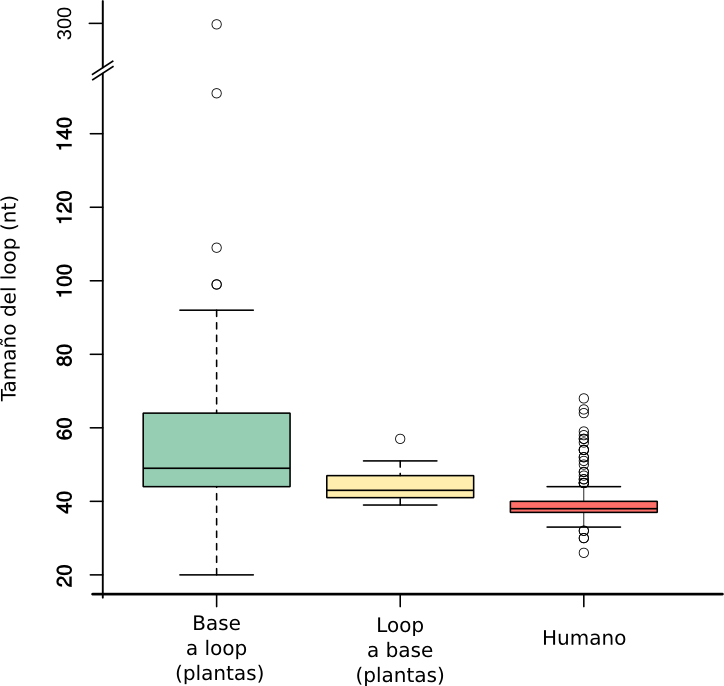
\includegraphics[width=0.7\textwidth]{loop_size.png}
	%~ \caption[Tamaño del loop terminal en precursores de distintos reinos]{
		%~ \textbf{Tamaño del loop terminal en precursores de distintos reinos}.
		%~ Se muestra la distribución del tamaño del loop terminal (nt) de precursores de plantas cortos de base a loop, en cortos de loop a base y de humanos.
		%~ Por simplicidad se utilizaron precursores de humanos conservados en 8 especies según nuestro criterio de búsqueda de ortólogos.
	%~ }
	%~ \label{fig:loop_size}
%~ \end{figure}

En animales, la estructura secundaria del loop terminal de precursores de miARNs, es irrelevante durante el procesamiento e inclusive se demostró que la presencia del mismo es innecesaria para el procesamiento por DROSHA \citep{pmid16751099}.
Sin embargo, la estructura del loop es importante para que los pre-miARNs sean exportados del nucleo al citoplasma, donde DICER produce el segundo corte que libera a los miARNs en animales.
El mecanismo de procesamiento en animales es similar al mecanismo de procesamiento de los precursores de plantas cortos de base a loop.
Sin embargo, podemos observar que estructuralmente los precursores en animales comparten patrones similares a los precursores de plantas cortos de loop a base y también a los cortos de la base al loop (Figura \ref{fig:animals_vs_plants_circos}) .
Esto se debería a que en animales existen determinantes para guiar a DROSHA (por debajo del miARN) y otros determinantes necesarios para que se exporte el precursor al citoplasma, donde DCL1 produce el segundo corte.


\begin{landscape} 
\begin{figure}[htbp!] 
        \centering    
        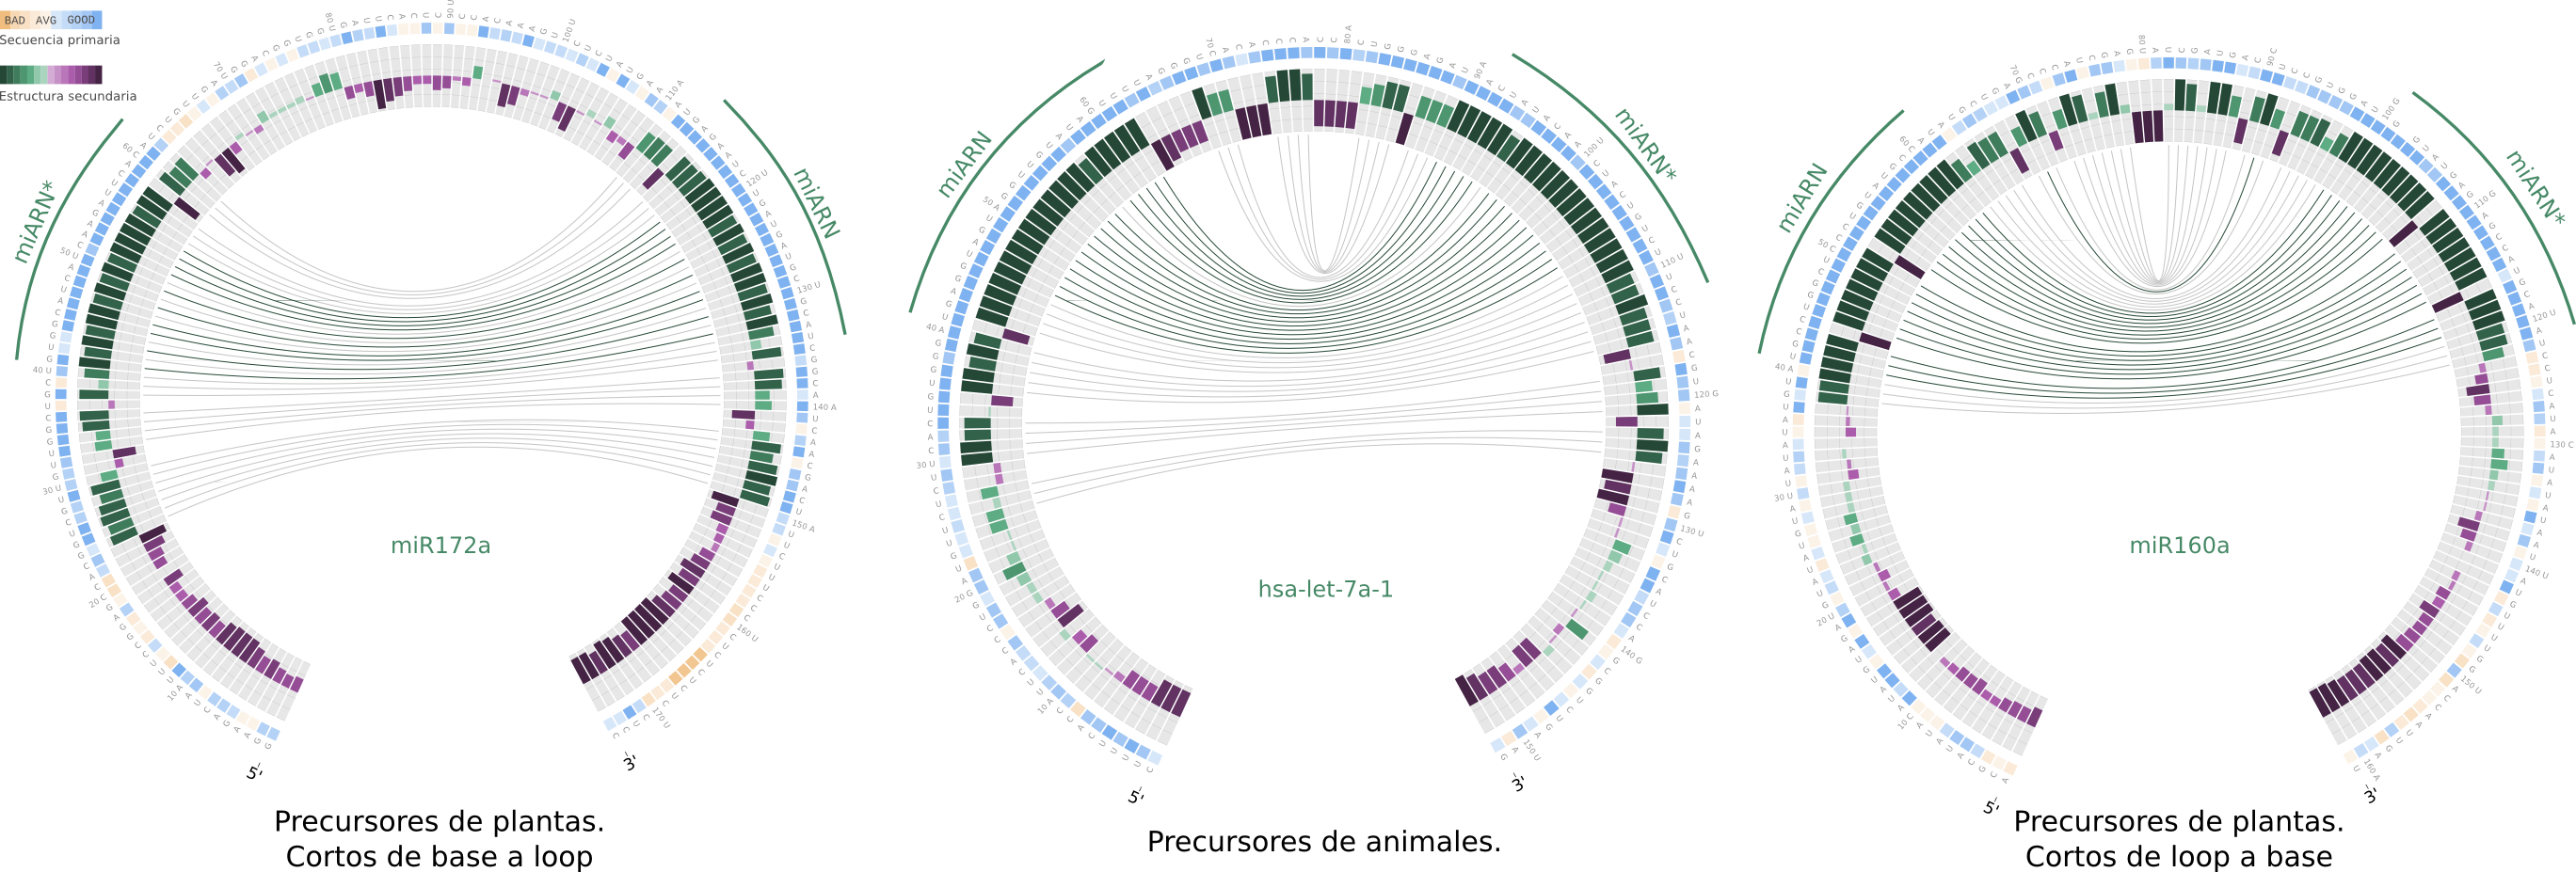
\includegraphics[width=1.4\textwidth]{animals_vs_plants_circos.png}
        \caption[Circos de animales vs plantas]{
        \textbf{Circos de animales vs plantas.}
		A la izquierda el Circos del miR172a, un precursor conservado en plantas con mecanismo corto de base a loop.
		En el medio el Circos del precursor de miARN de humano let-7a-1.
		A la derecha el Circos del miR160a, un precursor conservado en plantas con mecanismo corto de loop a base.
        }
	 \label{fig:animals_vs_plants_circos}
    \end{figure}
\end{landscape}


\section{Conclusiones.}
En esta parte del proyecto de Tesis presentamos un enfoque bioinformático para el estudio de la evolución y biogénesis de miARNs en plantas.
Para esto desarrollamos una implementación gráfica para visualizar de manera simple los precursores de miARNs en distintas especies de plantas.
Y fueron utilizados para caracterizar la evolución de precursores de miARNs en plantas con distintos mecanismos de procesamiento.
En el Anexo (Figuras \ref{fig:circos_all_01},\ref{fig:circos_all_02},\ref{fig:circos_all_03},\ref{fig:circos_all_04} y \ref{fig:circos_all_05}) se muestran los Circos de dicotiledóneas donde se detectan ortólogos en más de 20 especies de las 30 analizadas.

Esta metodología y visualización con Circos, la utilizamos para comparar precursores de miARNs de distintas familias y además en precursores de miARNs de distintos reinos.
En particular, estudiamos precursores con mutaciones puntuales que afectan al procesamiento de miARNs en plantas.
Y vimos, que la información obtenida de estos estudios, podria ser utilizada para ayudar en el diseño de miARNs artificiales en distintas especies y aumentar su eficiencia.

Si bien la biogénesis y modo de acción de precursores de animales es diferente a la de los precursores de plantas, pudimos utilizar este mismo enfoque para estudiar precursores de miARNs en animales.
Y pudimos observar que estructuralmente los precursores en animales comparten patrones similares a los precursores de plantas cortos de loop a base y también a los cortos de la base al loop.
Esto podría ser debido a que en animales existen determinantes para guiar a DROSHA (por debajo del miARN) y otros determinantes para que el exporte al citoplasma (por encima del miARN).
